\documentclass[11pt]{article}
\usepackage[utf8]{inputenc}
\usepackage{geometry}
\geometry{a4paper, margin=1in}
\usepackage{amsmath, amssymb, amsthm}
\usepackage{graphicx}
\usepackage{hyperref}
\usepackage{parskip}
\usepackage{xcolor}
\usepackage{tikz}
\usetikzlibrary{shapes, arrows, positioning, calc}

% --- Awesome Box Definitions ---
\usepackage[most]{tcolorbox}

% Question Box
\newtcolorbox[auto counter, number within=section]{questionbox}[2][]{%
    colback=blue!5!white,
    colframe=blue!75!black,
    fonttitle=\bfseries,
    title=Question~\thetcbcounter: #2,
    #1
}

% Solution Box
\newtcolorbox{solutionbox}[1][]{%
    colback=green!5!white,
    colframe=green!60!black,
    fonttitle=\bfseries,
    title=Solution,
    #1
}

\title{\textbf{\Huge Machine Learning Practice Problems}\\ \Large Comprehensive Set with Detailed Solutions}
\author{\textit{Prepared for Students}}
\date{\today}

\begin{document}

\maketitle
\tableofcontents
\newpage
\section{Introduction and Machine Learning Workflow}

\begin{questionbox}{Conceptual}
A credit card company wants to detect fraudulent transactions... (Supervised vs Unsupervised)
\end{questionbox}

\begin{solutionbox}
The first scenario is **Supervised Learning** (Classification)... The second is **Unsupervised Learning** (Anomaly Detection)...
\end{solutionbox}

\begin{questionbox}{Numerical}
Given feature $X=\{10, 20, 30, 40, 50\}$, Min-Max normalize 30.
\end{questionbox}

\begin{solutionbox}
$X_{norm} = \frac{30-10}{50-10} = 0.5$.
\end{solutionbox}

\begin{questionbox}{Numerical}
Dataset mean $\mu=100$, $\sigma=20$. Z-score for $x=130$.
\end{questionbox}

\begin{solutionbox}
$z = \frac{130-100}{20} = 1.5$. It is 1.5 std deviations above mean.
\end{solutionbox}

\begin{questionbox}{Conceptual}
Explain Curse of Dimensionality impact on KNN.
\end{questionbox}

\begin{solutionbox}
In high dimensions, distance becomes less meaningful (points become equidistant). KNN fails to distinguish neighbors.
\end{solutionbox}

\begin{questionbox}{Numerical}
PCA Eigenvalues $\lambda_1=4, \lambda_2=2, \lambda_3=0.5$. Variance explained by first two?
\end{questionbox}

\begin{solutionbox}
Total = 6.5. PC1+PC2 = 6.0. Prop = $6.0/6.5 \approx 92.3\%$.
\end{solutionbox}

\begin{questionbox}{Conceptual}
Why split into Train/Validation/Test?
\end{questionbox}

\begin{solutionbox}
Train: Fit parameters. Validation: Tune hyperparameters (prevent leakage). Test: Final evaluation.
\end{solutionbox}

\begin{questionbox}{Conceptual}
Handling Imbalanced Data (1\% positive).
\end{questionbox}

\begin{solutionbox}
1. Resampling (SMOTE, Undersampling). 2. Cost-sensitive learning.
\end{solutionbox}

\begin{questionbox}{Numerical}
Impute $F=\{2, 4, NaN, 8, 10, NaN\}$ with Median.
\end{questionbox}

\begin{solutionbox}
Observed: $\{2,4,8,10\}$. Median = 6. Imputed: $\{2,4,6,8,10,6\}$.
\end{solutionbox}

\begin{questionbox}{Conceptual}
Train Acc 99\%, Val Acc 65\%. Diagnosis?
\end{questionbox}

\begin{solutionbox}
**Overfitting**. Fixes: Pruning, Regularization, More Data.
\end{solutionbox}

\begin{questionbox}{Scenario}
Scaling for KNN vs Decision Trees?
\end{questionbox}

\begin{solutionbox}
Critical for **KNN** (distance based). Not required for **Decision Trees** (univariate splits).
\end{solutionbox}

\section{Linear Models for Regression}

\begin{questionbox}{Numerical}
Least Squares line for $(1,2), (2,3), (3,5)$.
\end{questionbox}

\begin{solutionbox}
Means: $\bar{x}=2, \bar{y}=3.33$. Slope $w_1 = \frac{3.0}{2.0} = 1.5$. Intercept $w_0 = 3.33 - 1.5(2) = 0.33$. Line: $y = 1.5x + 0.33$.
\end{solutionbox}

\begin{questionbox}{Numerical}
Gradient Descent step for $y=wx$. Data $(2,4)$, $w_{old}=1$, $\eta=0.1$.
\end{questionbox}

\begin{solutionbox}
Pred=2. Err=-2. Grad = $(-2)(2) = -4$. $w_{new} = 1 - 0.1(-4) = 1.4$.
\end{solutionbox}

\begin{questionbox}{Conceptual}
L1 (Lasso) vs L2 (Ridge).
\end{questionbox}

\begin{solutionbox}
Lasso can shrink weights to zero (Feature Selection). Ridge shrinks towards zero (Stability).
\end{solutionbox}

\begin{questionbox}{Numerical}
Ridge Cost: $w=[3,4]$, MSE=10, $\lambda=0.5$.
\end{questionbox}

\begin{solutionbox}
Reg = $0.5(3^2+4^2) = 12.5$. Total = $22.5$.
\end{solutionbox}

\begin{questionbox}{Scenario}
Poly Regression Degree 1 vs 20 for 50 points. Bias/Variance?
\end{questionbox}

\begin{solutionbox}
Deg 1: High Bias (Underfitting). Deg 20: High Variance (Overfitting).
\end{solutionbox}

\begin{questionbox}{Conceptual}
Batch vs Stochastic Gradient Descent.
\end{questionbox}

\begin{solutionbox}
Batch: Smooth, slow per step. SGD: Noisy, fast updates.
\end{solutionbox}

\begin{questionbox}{Numerical}
R-squared calculation: SSR=20, SST=100.
\end{questionbox}

\begin{solutionbox}
$R^2 = 1 - 20/100 = 0.8$.
\end{solutionbox}

\begin{questionbox}{Conceptual}
Effect of Learning Rate size.
\end{questionbox}

\begin{solutionbox}
Too large: Diverge/Overshoot. Too small: Slow convergence.
\end{solutionbox}

\begin{questionbox}{Scenario}
Modeling quadratic relationship with linear regression.
\end{questionbox}

\begin{solutionbox}
Basis Expansion: Add $x^2$ as feature.
\end{solutionbox}

\begin{questionbox}{Conceptual}
Elastic Net usage.
\end{questionbox}

\begin{solutionbox}
High correlation features or $p > n$. Combines L1 selection + L2 grouping.
\end{solutionbox}

\section{Linear Models for Classification}

\begin{questionbox}{Numerical}
Logistic Regression: $z=-2$. Predict $\hat{y}$.
\end{questionbox}

\begin{solutionbox}
$\sigma(-2) = 1/(1+e^2) \approx 0.119$.
\end{solutionbox}

\begin{questionbox}{Numerical}
Log Loss for $y=1, \hat{y}=0.8$.
\end{questionbox}

\begin{solutionbox}
$-\ln(0.8) \approx 0.223$.
\end{solutionbox}

\begin{questionbox}{Conceptual}
Why linear boundary in Logistic Regression?
\end{questionbox}

\begin{solutionbox}
Boundary is $w^Tx+b=0$, which is a hyperplane.
\end{solutionbox}

\begin{questionbox}{Numerical}
Odds Ratio for $w=0.5$.
\end{questionbox}

\begin{solutionbox}
$e^{0.5} \approx 1.65$. Odds increase by 65\%.
\end{solutionbox}

\begin{questionbox}{Conceptual}
Generative vs Discriminative (NB vs LR).
\end{questionbox}

\begin{solutionbox}
Gen (NB): Models $P(X,Y)$. Disc (LR): Models $P(Y|X)$ directly.
\end{solutionbox}

\begin{questionbox}{Scenario}
One-vs-Rest for 3 classes.
\end{questionbox}

\begin{solutionbox}
Train 3 classifiers: 1 vs Rest, 2 vs Rest, 3 vs Rest. Pick max probability.
\end{solutionbox}

\begin{questionbox}{Numerical}
Log-loss gradient for $x=2, y=1, \hat{y}=0.4$.
\end{questionbox}

\begin{solutionbox}
$(0.4 - 1)(2) = -1.2$.
\end{solutionbox}

\begin{questionbox}{Scenario}
Circular data with Logistic Regression?
\end{questionbox}

\begin{solutionbox}
Fails (linear). Needs feature engineering ($x_1^2 + x_2^2$).
\end{solutionbox}

\begin{questionbox}{Conceptual}
Assumption of Logistic Regression.
\end{questionbox}

\begin{solutionbox}
Linear relationship between features and log-odds.
\end{solutionbox}

\begin{questionbox}{Conceptual}
Effect of Regularization on boundary.
\end{questionbox}

\begin{solutionbox}
Smoother, simpler boundary. Reduces overfitting.
\end{solutionbox}

\section{Decision Tree Learning}

\begin{center}
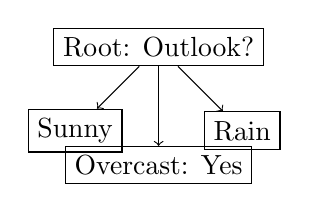
\begin{tikzpicture}[node distance=1.5cm]
\node (root) [rectangle, draw] {Root: Outlook?};
\node (sunny) [rectangle, draw, below left of=root] {Sunny};
\node (over) [rectangle, draw, below of=root] {Overcast: Yes};
\node (rain) [rectangle, draw, below right of=root] {Rain};
\draw [->] (root) -- (sunny);
\draw [->] (root) -- (over);
\draw [->] (root) -- (rain);
\end{tikzpicture}
\end{center}

\begin{questionbox}{Numerical}
Consider the following dataset for predicting whether a person will play tennis. Calculate the information gain for the attribute 'Wind' and 'Humidity'. Which attribute would the ID3 algorithm choose as the root of the tree?

\begin{center}
\begin{tabular}{|c|c|c|c|c|c|}
\hline
\textbf{Day} & \textbf{Outlook} & \textbf{Temperature} & \textbf{Humidity} & \textbf{Wind} & \textbf{Play Tennis} \\
\hline
D1 & Sunny & Hot & High & Weak & No \\
D2 & Sunny & Hot & High & Strong & No \\
D3 & Overcast & Hot & High & Weak & Yes \\
D4 & Rain & Mild & High & Weak & Yes \\
D5 & Rain & Cool & Normal & Weak & Yes \\
D6 & Rain & Cool & Normal & Strong & No \\
D7 & Overcast & Cool & Normal & Strong & Yes \\
D8 & Sunny & Mild & High & Weak & No \\
D9 & Sunny & Cool & Normal & Weak & Yes \\
D10 & Rain & Mild & Normal & Weak & Yes \\
D11 & Sunny & Mild & Normal & Strong & Yes \\
D12 & Overcast & Mild & High & Strong & Yes \\
D13 & Overcast & Hot & Normal & Weak & Yes \\
D14 & Rain & Mild & High & Strong & No \\
\hline
\end{tabular}
\end{center}
\end{questionbox}

\begin{solutionbox}
\textbf{Step 1: Calculate the entropy of the entire dataset.}
Out of 14 days, 9 are 'Yes' and 5 are 'No'.
$$ E(S) = - \frac{9}{14} \log_2\left(\frac{9}{14}\right) - \frac{5}{14} \log_2\left(\frac{5}{14}\right) \approx 0.940 $$

\textbf{Step 2: Calculate the information gain for 'Wind'.}
The 'Wind' attribute has two values: 'Weak' and 'Strong'.
For Wind = Weak: 8 days, 6 'Yes' and 2 'No'.
$$ E(\text{Wind=Weak}) = - \frac{6}{8} \log_2\left(\frac{6}{8}\right) - \frac{2}{8} \log_2\left(\frac{2}{8}\right) \approx 0.811 $$
For Wind = Strong: 6 days, 3 'Yes' and 3 'No'.
$$ E(\text{Wind=Strong}) = - \frac{3}{6} \log_2\left(\frac{3}{6}\right) - \frac{3}{6} \log_2\left(\frac{3}{6}\right) = 1 $$
The information gain for 'Wind' is:
$$ Gain(S, \text{Wind}) = E(S) - \left[ \left(\frac{8}{14}\right)E(\text{Wind=Weak}) + \left(\frac{6}{14}\right)E(\text{Wind=Strong}) \right] $$
$$ Gain(S, \text{Wind}) = 0.940 - \left[ \left(\frac{8}{14}\right)(0.811) + \left(\frac{6}{14}\right)(1) \right] \approx 0.048 $$

\textbf{Step 3: Calculate the information gain for 'Humidity'.}
The 'Humidity' attribute has two values: 'High' and 'Normal'.
For Humidity = High: 7 days, 3 'Yes' and 4 'No'.
$$ E(\text{Humidity=High}) = - \frac{3}{7} \log_2\left(\frac{3}{7}\right) - \frac{4}{7} \log_2\left(\frac{4}{7}\right) \approx 0.985 $$
For Humidity = Normal: 7 days, 6 'Yes' and 1 'No'.
$$ E(\text{Humidity=Normal}) = - \frac{6}{7} \log_2\left(\frac{6}{7}\right) - \frac{1}{7} \log_2\left(\frac{1}{7}\right) \approx 0.592 $$
The information gain for 'Humidity' is:
$$ Gain(S, \text{Humidity}) = E(S) - \left[ \left(\frac{7}{14}\right)E(\text{Humidity=High}) + \left(\frac{7}{14}\right)E(\text{Humidity=Normal}) \right] $$
$$ Gain(S, \text{Humidity}) = 0.940 - \left[ \left(\frac{7}{14}\right)(0.985) + \left(\frac{7}{14}\right)(0.592) \right] \approx 0.151 $$

\textbf{Step 4: Compare the information gains.}
$$ Gain(S, \text{Humidity}) = 0.151 > Gain(S, \text{Wind}) = 0.048 $$
The ID3 algorithm would choose \textbf{Humidity} as the root of the tree because it has a higher information gain.
\end{solutionbox}

\begin{questionbox}{Numerical}
A dataset has a continuous-valued attribute, 'Temperature', with the following values for a binary classification problem:
\begin{center}
\begin{tabular}{|c|c|c|c|c|c|c|c|c|}
\hline
\textbf{Temperature} & 64 & 68 & 69 & 70 & 72 & 75 & 80 & 85 \\
\hline
\textbf{Class} & No & No & Yes & Yes & Yes & No & No & Yes \\
\hline
\end{tabular}
\end{center}
Determine the best split point for 'Temperature' using the information gain criterion.
\end{questionbox}

\begin{solutionbox}
\textbf{Step 1: Identify potential split points.}
The potential split points are the midpoints between consecutive sorted values where the class label changes.
Sorted temperatures: 64, 68, 69, 70, 72, 75, 80, 85
Class labels: No, No, Yes, Yes, Yes, No, No, Yes
The class label changes between (68, 69), (72, 75), and (80, 85).
Potential split points:
\begin{itemize}
    \item $(68+69)/2 = 68.5$
    \item $(72+75)/2 = 73.5$
    \item $(80+85)/2 = 82.5$
\end{itemize}

\textbf{Step 2: Calculate the entropy of the entire dataset.}
There are 8 data points, 4 'Yes' and 4 'No'.
$$ E(S) = - \frac{4}{8} \log_2\left(\frac{4}{8}\right) - \frac{4}{8} \log_2\left(\frac{4}{8}\right) = 1 $$

\textbf{Step 3: Calculate the information gain for each split point.}
\begin{itemize}
    \item \textbf{Split at 68.5:}
    \begin{itemize}
        \item $T \le 68.5$: 2 points (No, No) -> $E = 0$
        \item $T > 68.5$: 6 points (Yes, Yes, Yes, No, No, Yes) -> 4 'Yes', 2 'No'
        $$ E(T>68.5) = - \frac{4}{6} \log_2\left(\frac{4}{6}\right) - \frac{2}{6} \log_2\left(\frac{2}{6}\right) \approx 0.918 $$
        $$ Gain(S, T_{68.5}) = 1 - \left[ \left(\frac{2}{8}\right)(0) + \left(\frac{6}{8}\right)(0.918) \right] \approx 0.311 $$
    \end{itemize}
    \item \textbf{Split at 73.5:}
    \begin{itemize}
        \item $T \le 73.5$: 5 points (No, No, Yes, Yes, Yes) -> 3 'Yes', 2 'No'
        $$ E(T \le 73.5) = - \frac{3}{5} \log_2\left(\frac{3}{5}\right) - \frac{2}{5} \log_2\left(\frac{2}{5}\right) \approx 0.971 $$
        \item $T > 73.5$: 3 points (No, No, Yes) -> 1 'Yes', 2 'No'
        $$ E(T > 73.5) = - \frac{1}{3} \log_2\left(\frac{1}{3}\right) - \frac{2}{3} \log_2\left(\frac{2}{3}\right) \approx 0.918 $$
        $$ Gain(S, T_{73.5}) = 1 - \left[ \left(\frac{5}{8}\right)(0.971) + \left(\frac{3}{8}\right)(0.918) \right] \approx 0.049 $$
    \end{itemize}
    \item \textbf{Split at 82.5:}
    \begin{itemize}
        \item $T \le 82.5$: 7 points (No, No, Yes, Yes, Yes, No, No) -> 3 'Yes', 4 'No'
        $$ E(T \le 82.5) = - \frac{3}{7} \log_2\left(\frac{3}{7}\right) - \frac{4}{7} \log_2\left(\frac{4}{7}\right) \approx 0.985 $$
        \item $T > 82.5$: 1 point (Yes) -> $E = 0$
        $$ Gain(S, T_{82.5}) = 1 - \left[ \left(\frac{7}{8}\right)(0.985) + \left(\frac{1}{8}\right)(0) \right] \approx 0.138 $$
    \end{itemize}
\end{itemize}

\textbf{Step 4: Choose the best split point.}
Comparing the information gains:
\begin{itemize}
    \item $Gain(S, T_{68.5}) \approx 0.311$
    \item $Gain(S, T_{73.5}) \approx 0.049$
    \item $Gain(S, T_{82.5}) \approx 0.138$
\end{itemize}
The best split point for 'Temperature' is \textbf{68.5}, as it provides the highest information gain.
\end{solutionbox}

\begin{questionbox}{Scenario-based}
A hospital wants to build a decision tree to predict the risk of a patient developing a certain disease. The available attributes are age, gender, blood pressure, cholesterol level, and whether the patient is a smoker. Some patients have missing values for their cholesterol level. How would you handle these missing values during the construction and classification phases of the decision tree?
\end{questionbox}

\begin{solutionbox}
\textbf{Handling Missing Values in Decision Trees:}

\textbf{During Tree Construction (at a node where 'cholesterol level' is the splitting attribute):}
\begin{enumerate}
    \item \textbf{Probabilistic Split:} When calculating the information gain for the 'cholesterol level' attribute, we can distribute the instances with missing values among the branches of the node. The distribution is proportional to the number of instances that have known values for that attribute. For example, if 70\% of the patients with known cholesterol levels have 'high' cholesterol and 30\% have 'normal' cholesterol, we would send 70\% of the patient with a missing cholesterol value down the 'high' branch and 30\% down the 'normal' branch. This allows us to use the information from the other attributes of these patients.
\end{enumerate}

\textbf{During Classification (when a new patient with a missing cholesterol level needs to be classified):}
\begin{enumerate}
    \item \textbf{Probabilistic Classification:} When the decision tree reaches a node that splits on 'cholesterol level', and the patient's cholesterol level is unknown, we can explore both branches of the tree. We then combine the classification results from both branches, weighted by the proportion of training instances that went down each branch. For example, if the 'high' cholesterol branch leads to a 'high risk' prediction with a probability of 0.8, and the 'normal' cholesterol branch leads to a 'low risk' prediction with a probability of 0.9, and the training data was split 70/30, the final prediction would be a weighted average of these outcomes.

    \item \textbf{Surrogate Splits:} Another approach is to use surrogate splits. At each node, in addition to the primary splitting attribute, we can identify other attributes that have similar splitting behavior. If a patient has a missing value for the primary attribute ('cholesterol level'), we can use the best surrogate split to decide which branch to follow. For instance, if 'age' is a good surrogate for 'cholesterol level', we would use the patient's age to make the split.
\end{enumerate}
\end{solutionbox}

\begin{questionbox}{Scenario-based}
You are tasked with building a decision tree for a credit scoring application. The goal is to predict whether a loan applicant is a high-risk or low-risk customer. What are the potential dangers of overfitting in this scenario, and what pre-pruning and post-pruning techniques could you employ to mitigate this risk?
\end{questionbox}

\begin{solutionbox}
\textbf{Dangers of Overfitting in Credit Scoring:}
An overfitted decision tree in this context would be one that has learned the training data too well, including its noise and outliers. This can lead to:
\begin{itemize}
    \item \textbf{Poor Generalization:} The model will perform poorly on new, unseen loan applicants because it has not learned the underlying patterns of credit risk but has instead memorized the training data.
    \item \textbf{Incorrect Risk Assessment:} This can lead to approving high-risk applicants who are likely to default (resulting in financial losses for the lender) or rejecting low-risk applicants who would have been good customers (resulting in lost business).
    \item \textbf{Model Instability:} Small changes in the training data could lead to a completely different tree, making the model unreliable.
\end{itemize}

\textbf{Mitigation Techniques:}

\textbf{Pre-pruning (stopping the tree from growing):}
\begin{enumerate}
    \item \textbf{Maximum Depth:} Set a limit on the maximum depth of the tree. This prevents the tree from becoming too complex and capturing noise in the data.
    \item \textbf{Minimum Samples for Split:} Do not split a node if the number of samples in it is below a certain threshold. This avoids creating splits based on a small number of instances, which are likely to be noise.
    \item \textbf{Minimum Samples for Leaf:} A node will not be split if, after the split, any of the resulting child nodes have fewer samples than a specified threshold.
    \item \textbf{Information Gain Threshold:} Only split a node if the information gain from the split is above a certain threshold.
\end{enumerate}

\textbf{Post-pruning (growing the tree fully and then trimming it):}
\begin{enumerate}
    \item \textbf{Reduced Error Pruning:} This is one of the simplest post-pruning methods. It involves using a validation set to evaluate the effect of pruning. For each node, we consider replacing the subtree rooted at that node with a single leaf node. If the error on the validation set does not increase, we perform the pruning.
    \item \textbf{Cost Complexity Pruning (Weakest Link Pruning):} This method, used in CART, involves considering a sequence of trees, each a subtree of the previous one. A complexity parameter, $\alpha$, is used to penalize the size of the tree. For each $\alpha$, we find the subtree that minimizes the sum of the misclassification rate and $\alpha$ times the number of leaves. Cross-validation is then used to find the optimal value of $\alpha$.
\end{enumerate}
\end{solutionbox}

\begin{questionbox}{Conceptual}
Explain the Minimum Description Length (MDL) principle and how it relates to avoiding overfitting in decision trees.
\end{questionbox}

\begin{solutionbox}
The \textbf{Minimum Description Length (MDL)} principle is a formalization of Occam's Razor. It states that the best hypothesis (or model) for a given set of data is the one that leads to the shortest description of the data. The total description length is the sum of two parts:
\begin{enumerate}
    \item \textbf{The length of the description of the hypothesis (the model).}
    \item \textbf{The length of the description of the data, given the hypothesis.}
\end{enumerate}

\textbf{Relation to Overfitting in Decision Trees:}

In the context of decision trees, the MDL principle can be used to decide when to stop growing the tree, thus avoiding overfitting.
\begin{itemize}
    \item \textbf{Hypothesis Description Length:} The description of the decision tree itself. A more complex tree (with more nodes and leaves) will have a longer description length.
    \item \textbf{Data Description Length (given the hypothesis):} This refers to the number of bits required to describe the classification of the training examples, given the tree. If the tree perfectly classifies the training data, this part of the description might be very short (or even zero). However, a simpler tree might misclassify some examples, and we would need to encode these exceptions, leading to a longer description of the data.
\end{itemize}

The MDL principle seeks to find a tree that minimizes the sum of these two description lengths.
\begin{itemize}
    \item A very simple tree will have a short hypothesis description but a long data description (due to many misclassifications).
    \item A very complex, overfitted tree will have a long hypothesis description but a short data description (as it fits the training data perfectly).
\end{itemize}

By applying the MDL principle, we aim for a balance. We stop growing the tree at a point where adding more nodes would increase the total description length. This typically happens when the increase in the complexity of the tree (longer hypothesis description) is not offset by a sufficient decrease in the number of misclassifications (shorter data description). In essence, MDL provides a principled way to trade off model complexity against training set accuracy, which is the core idea behind avoiding overfitting.
\end{solutionbox}

\begin{questionbox}{Numerical}
Calculate Gini for 10 Class A, 20 Class B.
\end{questionbox}

\begin{solutionbox}
$1 - ( (1/3)^2 + (2/3)^2 ) \approx 0.444$.
\end{solutionbox}

\begin{questionbox}{Conceptual}
Gini vs Entropy computation.
\end{questionbox}

\begin{solutionbox}
Gini avoids log, faster.
\end{solutionbox}

\begin{questionbox}{Conceptual}
Gain Ratio vs Information Gain.
\end{questionbox}

\begin{solutionbox}
Gain Ratio penalizes high-cardinality attributes (like ID).
\end{solutionbox}

\section{Instance-based Learning}

\begin{questionbox}{Numerical}
Given the following 2D data points for a binary classification problem, classify the new point (3, 4) using the k-Nearest Neighbor algorithm with k=3 and Euclidean distance.

\begin{center}
\begin{tabular}{|c|c|c|c|}
\hline
\textbf{Point} & \textbf{X} & \textbf{Y} & \textbf{Class} \\
\hline
P1 & 1 & 2 & A \\
P2 & 2 & 3 & A \\
P3 & 3 & 2 & B \\
P4 & 5 & 6 & B \\
P5 & 6 & 5 & B \\
P6 & 1 & 5 & A \\
\hline
\end{tabular}
\end{center}
\end{questionbox}

\begin{solutionbox}
\textbf{Step 1: Calculate the Euclidean distance from the new point (3, 4) to all other points.}
The Euclidean distance between two points $(x_1, y_1)$ and $(x_2, y_2)$ is $\sqrt{(x_2 - x_1)^2 + (y_2 - y_1)^2}$.

\begin{itemize}
    \item Distance to P1(1, 2): $\sqrt{(3-1)^2 + (4-2)^2} = \sqrt{4+4} = \sqrt{8} \approx 2.83$
    \item Distance to P2(2, 3): $\sqrt{(3-2)^2 + (4-3)^2} = \sqrt{1+1} = \sqrt{2} \approx 1.41$
    \item Distance to P3(3, 2): $\sqrt{(3-3)^2 + (4-2)^2} = \sqrt{0+4} = \sqrt{4} = 2.00$
    \item Distance to P4(5, 6): $\sqrt{(3-5)^2 + (4-6)^2} = \sqrt{4+4} = \sqrt{8} \approx 2.83$
    \item Distance to P5(6, 5): $\sqrt{(3-6)^2 + (4-5)^2} = \sqrt{9+1} = \sqrt{10} \approx 3.16$
    \item Distance to P6(1, 5): $\sqrt{(3-1)^2 + (4-5)^2} = \sqrt{4+1} = \sqrt{5} \approx 2.24$
\end{itemize}

\textbf{Step 2: Find the k=3 nearest neighbors.}
The distances in ascending order are:
\begin{enumerate}
    \item 1.41 (P2, Class A)
    \item 2.00 (P3, Class B)
    \item 2.24 (P6, Class A)
    \item 2.83 (P1, Class A)
    \item 2.83 (P4, Class B)
    \item 3.16 (P5, Class B)
\end{enumerate}
The 3 nearest neighbors are P2, P3, and P6.

\textbf{Step 3: Determine the class of the new point by majority vote.}
The classes of the 3 nearest neighbors are A, B, and A.
There are two 'A's and one 'B'. By majority vote, the new point (3, 4) is classified as \textbf{Class A}.
\end{solutionbox}

\begin{questionbox}{Numerical}
Repeat the previous question, but this time use Manhattan distance instead of Euclidean distance to classify the new point (3, 4) with k=3.
\end{questionbox}

\begin{solutionbox}
\textbf{Step 1: Calculate the Manhattan distance from the new point (3, 4) to all other points.}
The Manhattan distance between two points $(x_1, y_1)$ and $(x_2, y_2)$ is $|x_2 - x_1| + |y_2 - y_1|$.

\begin{itemize}
    \item Distance to P1(1, 2): $|3-1| + |4-2| = 2 + 2 = 4$
    \item Distance to P2(2, 3): $|3-2| + |4-3| = 1 + 1 = 2$
    \item Distance to P3(3, 2): $|3-3| + |4-2| = 0 + 2 = 2$
    \item Distance to P4(5, 6): $|3-5| + |4-6| = 2 + 2 = 4$
    \item Distance to P5(6, 5): $|3-6| + |4-5| = 3 + 1 = 4$
    \item Distance to P6(1, 5): $|3-1| + |4-5| = 2 + 1 = 3$
\end{itemize}

\textbf{Step 2: Find the k=3 nearest neighbors.}
The distances in ascending order are:
\begin{enumerate}
    \item 2 (P2, Class A)
    \item 2 (P3, Class B)
    \item 3 (P6, Class A)
    \item 4 (P1, Class A)
    \item 4 (P4, Class B)
    \item 4 (P5, Class B)
\end{enumerate}
The 3 nearest neighbors are P2, P3, and P6.

\textbf{Step 3: Determine the class of the new point by majority vote.}
The classes of the 3 nearest neighbors are A, B, and A.
There are two 'A's and one 'B'. By majority vote, the new point (3, 4) is classified as \textbf{Class A}.
\end{solutionbox}

\begin{questionbox}{Scenario-based}
You are working on a real estate price prediction model. You have a dataset with features like square footage, number of bedrooms, location, and age of the house. You decide to use Locally Weighted Regression (LWR). How does LWR differ from standard linear regression, and why might it be a good choice for this problem?
\end{questionbox}

\begin{solutionbox}
\textbf{Difference between LWR and Standard Linear Regression:}
\begin{itemize}
    \item \textbf{Global vs. Local Model:} Standard linear regression is a global model. It learns a single set of parameters (coefficients) for the entire dataset, trying to find a linear relationship that best fits all the data points. In contrast, LWR is a local model. It does not learn a fixed set of parameters. Instead, for each new query point for which we want to make a prediction, it fits a separate linear regression model to a localized subset of the training data around that query point.
    \item \textbf{Weighting of Data Points:} In standard linear regression, all training examples have an equal influence on the final model. In LWR, the training examples are weighted based on their proximity to the query point. Points closer to the query point are given a higher weight, and points farther away are given a lower weight. This is typically done using a kernel function (e.g., a Gaussian kernel).
    \item \textbf{Computational Cost:} Standard linear regression is computationally efficient. Once the model is trained, predictions are very fast. LWR has a higher computational cost at prediction time because a new regression model has to be fit for every single prediction.
\end{itemize}

\textbf{Why LWR might be a good choice for real estate price prediction:}
The relationship between house features and price is often non-linear and can vary in different parts of the feature space.
\begin{itemize}
    \item \textbf{Non-linearity:} The price per square foot might be different for small apartments versus large mansions. The impact of the number of bedrooms on the price might not be linear (the fifth bedroom might add less value than the third). LWR can capture these non-linearities by fitting local linear models.
    \item \textbf{Location Dependence:} The relationship between features and price can be highly dependent on the location. For example, the age of a house might be a positive factor in a historic neighborhood but a negative factor in a newer suburb. LWR can adapt to these local variations. For a query point in a specific neighborhood, it will give more weight to the houses in that same neighborhood, effectively learning a local pricing model.
\end{itemize}
In summary, LWR is a good choice for this problem because it can model the complex, non-linear, and locally varying relationships that are common in real estate markets.
\end{solutionbox}

\begin{questionbox}{Scenario-based}
Explain the "curse of dimensionality" and its impact on the k-Nearest Neighbor algorithm. How can this problem be addressed?
\end{questionbox}

\begin{solutionbox}
\textbf{The Curse of Dimensionality:}
The "curse of dimensionality" refers to various phenomena that arise when analyzing and organizing data in high-dimensional spaces that do not occur in low-dimensional settings. As the number of features (dimensions) increases, the volume of the space increases so fast that the available data becomes sparse. This sparsity is problematic for any method that requires statistical significance.

\textbf{Impact on k-NN:}
The k-NN algorithm relies on the assumption that points that are close to each other in the feature space are likely to belong to the same class. The "closeness" is measured by a distance metric like Euclidean distance. In high dimensions, this assumption breaks down:
\begin{itemize}
    \item \textbf{Distance Concentration:} In high-dimensional spaces, the distances between all pairs of points tend to become very similar. The concept of a "nearest" neighbor becomes less meaningful because the distance to the nearest neighbor can be comparable to the distance to the farthest neighbor.
    \item \textbf{Sparsity:} To maintain the same density of data points as the number of dimensions increases, we need an exponentially increasing number of data points. With a fixed number of data points, the space becomes very sparse, and the nearest neighbors can be very far away.
    \item \textbf{Irrelevant Features:} In high-dimensional data, it is likely that many of the features are irrelevant to the classification task. These irrelevant features can add noise to the distance calculations, making it harder to find the true nearest neighbors.
\end{itemize}

\textbf{Addressing the Problem:}
\begin{enumerate}
    \item \textbf{Dimensionality Reduction:} This is the most common approach. Techniques like Principal Component Analysis (PCA) or Linear Discriminant Analysis (LDA) can be used to project the data onto a lower-dimensional subspace while preserving as much of the relevant information as possible.
    \item \textbf{Feature Selection:} Instead of transforming the features, we can select a subset of the most relevant features and discard the rest. This can be done using various statistical tests or model-based selection methods.
    \item \textbf{Use of Different Distance Metrics:} Some distance metrics, like the cosine similarity, can be less sensitive to the curse of dimensionality in certain contexts (e.g., text data).
    \item \textbf{Increase the amount of training data:} While often impractical, having a very large amount of data can help to mitigate the effects of sparsity.
\end{enumerate}
\end{solutionbox}

\begin{questionbox}{Conceptual}
What are Radial Basis Functions (RBFs) and how are they used in instance-based learning?
\end{questionbox}

\begin{solutionbox}
A \textbf{Radial Basis Function (RBF)} is a real-valued function whose value depends only on the distance from the origin or from some other point, called a center. A common example of an RBF is the Gaussian function:
$$ \phi(r) = e^{-(\epsilon r)^2} $$
where $r$ is the radial distance and $\epsilon$ is a shape parameter.

\textbf{Use in Instance-based Learning (RBF Networks):}
RBFs are the building blocks of RBF networks, which are a type of artificial neural network used for function approximation and classification. An RBF network typically has three layers:
\begin{enumerate}
    \item \textbf{Input Layer:} This layer simply takes the input feature vector.
    \item \textbf{Hidden Layer:} This layer consists of a number of RBF neurons. Each neuron has a "center," which is a prototype vector from the training data. When a new input vector is presented to the network, each hidden neuron calculates the distance between the input and its center and applies the RBF to this distance. The output of the hidden neuron is a measure of the similarity between the input and the neuron's prototype.
    \item \textbf{Output Layer:} The output of the network is a linear combination of the outputs of the hidden neurons.
\end{enumerate}

In the context of instance-based learning, RBF networks can be seen as a generalization of k-NN. Instead of a simple majority vote from the nearest neighbors, an RBF network learns to combine the "votes" of all the training instances (or a subset of them represented by the RBF centers) in a more sophisticated, weighted manner. The weights are learned during the training process. The influence of each training instance is localized, meaning it has a strong effect on predictions for nearby points and a weak effect on predictions for faraway points, which is a key characteristic of instance-based learning.
\end{solutionbox}

\begin{questionbox}{Numerical}
Weighted KNN ($1/d^2$): $d_A=1, d_B=2, d_B=4$. Predict.
\end{questionbox}

\begin{solutionbox}
$w_A=1$. $w_B = 0.25+0.06=0.31$. Class A.
\end{solutionbox}

\begin{questionbox}{Conceptual}
Lazy Learner implication.
\end{questionbox}

\begin{solutionbox}
Fast train, slow predict.
\end{solutionbox}

\begin{questionbox}{Conceptual}
Manhattan vs Euclidean.
\end{questionbox}

\begin{solutionbox}
Manhattan for grid/city-block.
\end{solutionbox}

\section{Support Vector Machines (SVMs)}

\begin{center}
\begin{tikzpicture}
\draw[thick] (-2, -1) -- (2, 3) node[right] {Hyperplane};
\draw[dashed] (-2, 0) -- (2, 4) node[right] {Margin +};
\draw[dashed] (-1, -2) -- (3, 2) node[right] {Margin -};
\fill[blue] (0, 2) circle (2pt);
\fill[red] (1, 0) circle (2pt);
\end{tikzpicture}
\end{center}

\begin{questionbox}{Numerical}
Consider a dataset with two points from class +1 at (1, 1) and (2, 2), and two points from class -1 at (1, 3) and (2, 4). Can this data be separated by a linear SVM? If so, find the equation of the maximum margin hyperplane and the width of the margin.
\end{questionbox}

\begin{solutionbox}
\textbf{Step 1: Check for linear separability and identify support vectors.}
The points are Class +1: A=(1, 1), B=(2, 2) and Class -1: C=(1, 3), D=(2, 4). The data is linearly separable. By inspection, the closest points between the classes are B=(2, 2) and C=(1, 3). These will be our support vectors.

\textbf{Step 2: Define the hyperplane and margin equations.}
Let the hyperplane be $w \cdot x + b = 0$. For the support vectors, we have:
\begin{itemize}
    \item For B=(2, 2) (class +1): $w \cdot (2, 2) + b = 1 \implies 2w_1 + 2w_2 + b = 1$
    \item For C=(1, 3) (class -1): $w \cdot (1, 3) + b = -1 \implies w_1 + 3w_2 + b = -1$
\end{itemize}

\textbf{Step 3: Solve for w and b.}
Subtracting the second equation from the first: $(2w_1 - w_1) + (2w_2 - 3w_2) = 1 - (-1) \implies w_1 - w_2 = 2$.
The vector $w$ must be parallel to the vector connecting the support vectors B and C, which is $B - C = (2-1, 2-3) = (1, -1)$.
So, we can write $w = k(1, -1) = (k, -k)$ for some scalar $k$.
Substitute this into $w_1 - w_2 = 2$: $k - (-k) = 2 \implies 2k = 2 \implies k = 1$.
Therefore, $w = (1, -1)$.

Now substitute $w$ back into one of the margin equations to find $b$:
Using $2w_1 + 2w_2 + b = 1$: $2(1) + 2(-1) + b = 1 \implies 0 + b = 1 \implies b = 1$.

\textbf{Step 4: State the hyperplane equation and calculate the margin width.}
The equation of the maximum margin hyperplane is $w \cdot x + b = 0$, which is $1x_1 - 1x_2 + 1 = 0$ or $\mathbf{x_1 - x_2 + 1 = 0}$.
The width of the margin is given by $2 / ||w||$.
$||w|| = \sqrt{1^2 + (-1)^2} = \sqrt{2}$.
Margin width = $\mathbf{2 / \sqrt{2} = \sqrt{2}}$.
\end{solutionbox}

\begin{questionbox}{Numerical}
Consider a soft margin SVM. A data point $(2, 3)$ with label $y = +1$ is classified using the hyperplane $2x_1 - x_2 + 1 = 0$. What is the value of the slack variable $\xi$ for this point? Is the point correctly classified? Is it on the correct side of the margin?
\end{questionbox}

\begin{solutionbox}
\textbf{Step 1: Understand the soft margin constraint.}
The constraint for a soft margin SVM is $y_i(w \cdot x_i + b) \ge 1 - \xi_i$, with $\xi_i \ge 0$. The slack variable $\xi_i$ measures the degree of violation of the margin.

\textbf{Step 2: Identify the parameters.}
\begin{itemize}
    \item Data point $x_i = (2, 3)$
    \item Label $y_i = +1$
    \item Hyperplane: $2x_1 - x_2 + 1 = 0$. So, $w = (2, -1)$ and $b = 1$.
\end{itemize}

\textbf{Step 3: Calculate the value of the decision function for the point.}
$f(x_i) = w \cdot x_i + b = (2)(2) + (-1)(3) + 1 = 4 - 3 + 1 = 2$.

\textbf{Step 4: Determine the slack variable $\xi_i$.}
We plug the values into the constraint equation to find the minimum required $\xi_i$:
$y_i(w \cdot x_i + b) \ge 1 - \xi_i$
$(+1)(2) \ge 1 - \xi_i$
$2 \ge 1 - \xi_i$
$\xi_i \ge 1 - 2 \implies \xi_i \ge -1$.
Since we also have the constraint $\xi_i \ge 0$, the smallest possible value for $\xi_i$ is 0.
So, the slack variable $\mathbf{\xi = 0}$.

\textbf{Step 5: Analyze the classification.}
\begin{itemize}
    \item \textbf{Is it correctly classified?} The sign of $y_i \cdot f(x_i)$ is $(+1)(2) = +2$, which is positive. So, \textbf{yes, the point is correctly classified}.
    \item \textbf{Is it on the correct side of the margin?} For a point to be on or outside the correct margin, we need $y_i(w \cdot x_i + b) \ge 1$. Here, we have $(+1)(2) = 2$, which is $\ge 1$. So, \textbf{yes, the point is outside the margin on the correct side}. A slack variable of 0 indicates no violation of the margin.
\end{itemize}
\end{solutionbox}

\begin{questionbox}{Scenario-based}
You are working on a text classification problem to categorize news articles into topics like 'sports', 'politics', and 'technology'. Why would an SVM with a non-linear kernel (like a Gaussian RBF kernel) be a good choice for this task? Explain the role of the kernel trick.
\end{questionbox}

\begin{solutionbox}
\textbf{Why a non-linear SVM is suitable for text classification:}
Text data, when represented in a high-dimensional space (e.g., using a bag-of-words model), is often not linearly separable. The relationships between words and topics can be complex and non-linear. For example, the presence of the word 'apple' could indicate a 'technology' article or a 'food' article depending on the context. A linear classifier might struggle to capture these nuances. An SVM with a non-linear kernel can map the data into a higher-dimensional feature space where it becomes linearly separable, allowing for a more accurate classification.

\textbf{The Kernel Trick:}
The kernel trick is a powerful idea that allows us to use SVMs for non-linear classification without explicitly mapping the data to a higher-dimensional space.
\begin{enumerate}
    \item \textbf{The problem:} If we want to find a non-linear decision boundary, we can project our data into a higher-dimensional space where it becomes linearly separable. However, this explicit transformation can be computationally very expensive, especially if the new feature space has a very large or even infinite number of dimensions.
    \item \textbf{The solution:} The SVM algorithm only depends on the dot products of the data points, not the data points themselves. The kernel trick involves using a kernel function, $K(x_i, x_j)$, which computes the dot product of the transformed feature vectors, $\phi(x_i) \cdot \phi(x_j)$, without ever having to compute the transformation $\phi(x)$ itself.
\end{enumerate}
For example, the Gaussian RBF kernel is defined as $K(x_i, x_j) = \exp(-\gamma ||x_i - x_j||^2)$. This kernel corresponds to a mapping to an infinite-dimensional feature space. By using this kernel function, we can get the benefits of this high-dimensional space without the computational burden of working in it. This makes non-linear SVMs practical and powerful for tasks like text classification.
\end{solutionbox}

\begin{questionbox}{Scenario-based}
An e-commerce company wants to build a recommendation system. They have data on which products users have purchased. How could SVMs be applied to this problem, and what are the challenges?
\end{questionbox}

\begin{solutionbox}
\textbf{Application of SVMs to Recommendation Systems:}
SVMs can be used for recommendation systems, typically as a part of a collaborative filtering or content-based filtering approach. One common way is to frame the problem as a binary classification task for each user-item pair:
\begin{itemize}
    \item \textbf{Positive examples:} User-item pairs where the user has purchased or rated the item highly.
    \item \textbf{Negative examples:} User-item pairs where the user has not interacted with the item, or has rated it poorly.
    \item \textbf{Features:} The features for a user-item pair could include user features (demographics, past purchase history), item features (category, brand, price), and interaction features (e.g., the similarity between the current item and items the user has liked in the past).
\end{itemize}
An SVM can then be trained to predict whether a user will like a given item. The items with the highest prediction scores can then be recommended to the user.

\textbf{Challenges:}
\begin{enumerate}
    \item \textbf{Scalability:} Recommendation systems for e-commerce sites often have millions of users and items. Training an SVM on such a large dataset can be computationally very expensive, both in terms of time and memory.
    \item \textbf{Sparsity:} The user-item interaction matrix is typically very sparse, meaning that most users have only interacted with a small fraction of the available items. This can make it difficult for the SVM to learn meaningful patterns.
    \item \textbf{Cold Start Problem:} For new users or new items, there is little to no interaction data. This makes it difficult to generate features and make accurate predictions. SVMs, like many other machine learning models, struggle with this problem.
    \item \textbf{Generating Negative Samples:} It is not always clear how to select negative samples. Should we treat all unobserved user-item pairs as negative? This could introduce a lot of noise.
\end{enumerate}
While SVMs can be used for recommendations, other methods like matrix factorization are often more scalable and better suited to the collaborative filtering task.
\end{solutionbox}

\begin{questionbox}{Conceptual}
What is Mercer's theorem and why is it important for the kernel trick in SVMs?
\end{questionbox}

\begin{solutionbox}
\textbf{Mercer's Theorem:}
Mercer's theorem provides the mathematical foundation for the kernel trick. It specifies the conditions under which a function can be considered a valid kernel, meaning that it corresponds to a dot product in some higher-dimensional feature space.

The theorem states that a symmetric, continuous function $K(x, z)$ can be expressed as a dot product in a high-dimensional space, i.e., $K(x, z) = \phi(x) \cdot \phi(z)$, if and only if the kernel matrix, formed by evaluating the kernel function on any finite set of points, is positive semi-definite.

\textbf{Importance for the Kernel Trick:}
Mercer's theorem is crucial for SVMs because it gives us a way to design and validate kernel functions without having to explicitly define the mapping function $\phi(x)$.
\begin{itemize}
    \item \textbf{Validity Check:} It allows us to check if a function we want to use as a kernel is valid. If a function satisfies Mercer's conditions, we know that there exists a feature space where it acts as a dot product, even if we don't know what that space is.
    \item \textbf{Flexibility:} It gives us the freedom to design custom kernel functions for specific problems, as long as they satisfy the conditions of the theorem. This allows SVMs to be adapted to a wide range of data types and problem domains.
    \item \textbf{Theoretical Guarantee:} It provides the theoretical guarantee that the optimization problem of the SVM in the feature space has a unique solution, which is essential for the algorithm to work correctly.
\end{itemize}
In essence, Mercer's theorem is the key that unlocks the power of the kernel trick, allowing us to use SVMs to learn complex, non-linear decision boundaries in a computationally efficient manner.
\end{solutionbox}

\begin{questionbox}{Numerical}
Margin for $w=(3,4)$.
\end{questionbox}

\begin{solutionbox}
$2/5 = 0.4$.
\end{solutionbox}

\begin{questionbox}{Conceptual}
Hinge Loss intuition.
\end{questionbox}

\begin{solutionbox}
Zero if correct and outside margin. Linear penalty otherwise.
\end{solutionbox}

\begin{questionbox}{Conceptual}
Dual Formulation benefit.
\end{questionbox}

\begin{solutionbox}
Allows Kernel Trick via dot products.
\end{solutionbox}

\section{Bayesian Learning}

\begin{questionbox}{Numerical}
Consider the following dataset for classifying documents as 'Sports' or 'Not Sports'.
\begin{center}
\begin{tabular}{|c|c|c|c|c|}
\hline
\textbf{Doc ID} & \textbf{Contains 'game'} & \textbf{Contains 'player'} & \textbf{Contains 'tax'} & \textbf{Class} \\
\hline
1 & Yes & Yes & No & Sports \\
2 & No & Yes & No & Sports \\
3 & Yes & No & No & Sports \\
4 & No & Yes & Yes & Not Sports \\
5 & Yes & No & Yes & Not Sports \\
\hline
\end{tabular}
\end{center}
Using a Naïve Bayes classifier with Laplace smoothing (add-1 smoothing), classify the new document: "game player". What is the posterior probability for each class?
\end{questionbox}

\begin{solutionbox}
\textbf{Step 1: Calculate prior probabilities.}
Total documents = 5.
$P(\text{Sports}) = 3/5 = 0.6$
$P(\text{Not Sports}) = 2/5 = 0.4$

\textbf{Step 2: Calculate likelihoods with Laplace smoothing.}
The formula for likelihood with Laplace smoothing is $P(word|Class) = \frac{\text{count}(word, Class) + 1}{\text{count}(Class) + k}$, where $k$ is the vocabulary size.
Our vocabulary is {'game', 'player', 'tax'}, so $k=3$.

\textbf{For Class = Sports (3 documents):}
\begin{itemize}
    \item $P(\text{game}|\text{Sports}) = (2+1)/(3+3) = 3/6 = 0.5$
    \item $P(\text{player}|\text{Sports}) = (2+1)/(3+3) = 3/6 = 0.5$
    \item $P(\text{tax}|\text{Sports}) = (0+1)/(3+3) = 1/6 \approx 0.167$
\end{itemize}
The new document does not contain 'tax', so we need $P(\text{not tax}|\text{Sports}) = 1 - P(\text{tax}|\text{Sports}) = 5/6$.

\textbf{For Class = Not Sports (2 documents):}
\begin{itemize}
    \item $P(\text{game}|\text{Not Sports}) = (1+1)/(2+3) = 2/5 = 0.4$
    \item $P(\text{player}|\text{Not Sports}) = (1+1)/(2+3) = 2/5 = 0.4$
    \item $P(\text{tax}|\text{Not Sports}) = (2+1)/(2+3) = 3/5 = 0.6$
\end{itemize}
The new document does not contain 'tax', so we need $P(\text{not tax}|\text{Not Sports}) = 1 - P(\text{tax}|\text{Not Sports}) = 2/5 = 0.4$.

\textbf{Step 3: Calculate the posterior probability for the new document "game player".}
The new document has 'game'=Yes, 'player'=Yes, 'tax'=No.
\begin{itemize}
    \item $P(\text{Sports} | \text{doc}) \propto P(\text{Sports}) \cdot P(\text{game}|\text{Sports}) \cdot P(\text{player}|\text{Sports}) \cdot P(\text{not tax}|\text{Sports})$
    $ \propto 0.6 \cdot 0.5 \cdot 0.5 \cdot (5/6) = 0.125$

    \item $P(\text{Not Sports} | \text{doc}) \propto P(\text{Not Sports}) \cdot P(\text{game}|\text{Not Sports}) \cdot P(\text{player}|\text{Not Sports}) \cdot P(\text{not tax}|\text{Not Sports})$
    $ \propto 0.4 \cdot 0.4 \cdot 0.4 \cdot 0.4 = 0.0256$
\end{itemize}

\textbf{Step 4: Normalize to get the final probabilities.}
Normalization constant (evidence) $Z = 0.125 + 0.0256 = 0.1506$.
\begin{itemize}
    \item $P(\text{Sports} | \text{doc}) = 0.125 / 0.1506 \approx \mathbf{0.830}$
    \item $P(\text{Not Sports} | \text{doc}) = 0.0256 / 0.1506 \approx \mathbf{0.170}$
\end{itemize}
The classifier predicts the document as \textbf{Sports}.
\end{solutionbox}

\begin{questionbox}{Numerical}
You flip a thumbtack 10 times and it lands 'pins up' 7 times and 'pins down' 3 times. Let $\theta$ be the probability of it landing 'pins up'.
(a) What is the Maximum Likelihood Estimate (MLE) for $\theta$?
(b) Suppose you have a prior belief about the thumbtack, which can be modeled by a Beta distribution $Beta(\alpha=2, \beta=2)$. What is the Maximum a Posteriori (MAP) estimate for $\theta$?
\end{questionbox}

\begin{solutionbox}
\textbf{(a) Maximum Likelihood Estimate (MLE)}

\textbf{Step 1: Write the likelihood function.}
The data follows a binomial distribution. The likelihood of observing 7 heads (up) and 3 tails (down) in 10 trials is:
$$ L(\theta) = P(Data | \theta) = \binom{10}{7} \theta^7 (1-\theta)^3 $$

\textbf{Step 2: Maximize the likelihood.}
To maximize $L(\theta)$, we can maximize its logarithm, the log-likelihood $l(\theta)$:
$$ l(\theta) = \log\binom{10}{7} + 7\log(\theta) + 3\log(1-\theta) $$
Take the derivative with respect to $\theta$ and set it to zero:
$$ \frac{dl}{d\theta} = \frac{7}{\theta} - \frac{3}{1-\theta} = 0 $$
$$ \frac{7}{\theta} = \frac{3}{1-\theta} \implies 7(1-\theta) = 3\theta \implies 7 - 7\theta = 3\theta \implies 7 = 10\theta $$
$$ \theta_{MLE} = \frac{7}{10} = \mathbf{0.7} $$

\textbf{(b) Maximum a Posteriori (MAP) Estimate}

\textbf{Step 1: Define the posterior distribution.}
The posterior is proportional to the likelihood times the prior: $P(\theta | Data) \propto P(Data | \theta) P(\theta)$.
The prior is $P(\theta) \sim Beta(\alpha, \beta)$, so $P(\theta) \propto \theta^{\alpha-1}(1-\theta)^{\beta-1}$.
Here, $\alpha=2, \beta=2$.
$$ P(\theta | Data) \propto \left[\theta^7 (1-\theta)^3\right] \cdot \left[\theta^{2-1}(1-\theta)^{2-1}\right] = \theta^7 (1-\theta)^3 \cdot \theta^1 (1-\theta)^1 $$
$$ P(\theta | Data) \propto \theta^{7+1} (1-\theta)^{3+1} = \theta^8 (1-\theta)^4 $$
This is the kernel of a Beta distribution, $Beta(7+\alpha, 3+\beta) = Beta(9, 5)$.

\textbf{Step 2: Find the mode of the posterior distribution.}
For a Beta($\alpha'$, $\beta'$) distribution, the mode (which is the MAP estimate) is given by $(\alpha' - 1) / (\alpha' + \beta' - 2)$.
Here $\alpha' = 9, \beta' = 5$.
$$ \theta_{MAP} = \frac{9-1}{9+5-2} = \frac{8}{12} = \frac{2}{3} \approx \mathbf{0.667} $$
The prior belief of the tack being fair (centered at 0.5) has pulled the estimate down from the MLE of 0.7.
\end{solutionbox}

\begin{questionbox}{Scenario-based}
A medical research team is building a probabilistic model to diagnose a rare disease. They have a small but reliable dataset of patients. They are debating between using a Maximum Likelihood Estimation (MLE) or a Maximum a Posteriori (MAP) approach to estimate the model parameters. Which approach would you recommend and why? What kind of prior information might be useful in this scenario?
\end{questionbox}

\begin{solutionbox}
\textbf{Recommendation: MAP Estimation}

I would strongly recommend using the \textbf{Maximum a Posteriori (MAP)} approach. Here's why:
\begin{enumerate}
    \item \textbf{Small Dataset:} MLE is known to overfit when the dataset is small. The parameters estimated by MLE are solely based on the observed data. If the small dataset happens to contain some random fluctuations or is not perfectly representative, MLE will capture this noise. For example, if by chance no patients in the small dataset had a particular symptom, MLE would assign a probability of zero to that symptom, which is likely incorrect and would cause problems when classifying new patients.
    \item \textbf{Regularization Effect of Priors:} MAP incorporates a prior probability distribution over the parameters. This prior acts as a form of regularization. It allows the researchers to inject their domain knowledge or previous beliefs into the model, preventing the parameters from taking extreme values based only on the limited data. For a rare disease, this is crucial. The prior "pulls" the estimate towards a more reasonable value, leading to better generalization.
\end{enumerate}

\textbf{Useful Prior Information:}
The medical team could incorporate prior knowledge from various sources:
\begin{itemize}
    \item \textbf{Existing Medical Literature:} Previous studies on similar diseases could provide information about the expected prevalence of symptoms. This could be used to formulate an informative prior. For example, if literature suggests a certain symptom is typically present in 20\% of patients with similar conditions, they could use a Beta prior centered around 0.2.
    \item \textbf{Expert Opinion:} Doctors and specialists have years of experience. Their clinical intuition about the disease can be encoded into a prior distribution. For instance, they might believe that a certain test result is very unlikely to be positive for healthy individuals, allowing them to set a prior that penalizes high probabilities for that parameter.
    \item \textbf{General Principles:} Even without specific knowledge, they can use a weakly informative prior. For instance, using a simple Beta(2, 2) prior (as in the numerical question) expresses a slight belief that probabilities are more likely to be around 0.5 than 0 or 1, which is often a more reasonable starting point than the uniform prior assumed by MLE. This prevents probabilities from becoming exactly 0 or 1, a common issue with MLE on small datasets.
\end{itemize}
\end{solutionbox}

\begin{questionbox}{Scenario-based}
You are designing an email spam filter using a Naïve Bayes classifier.
(a) What features would you use to represent an email?
(b) Explain the "zero-frequency problem" in this context and how you would solve it.
\end{questionbox}

\begin{solutionbox}
\textbf{(a) Feature Representation for Emails:}

A common and effective way to represent an email for a Naïve Bayes classifier is the \textbf{Bag-of-Words (BoW)} model.
\begin{enumerate}
    \item \textbf{Tokenization:} First, the email text is broken down into individual words or "tokens".
    \item \textbf{Preprocessing:} These tokens are then preprocessed, which can include converting all words to lowercase, removing punctuation and special characters, and removing common "stop words" (like 'the', 'is', 'a', 'in') that don't carry much meaning. Stemming or lemmatization (reducing words to their root form, e.g., 'running' -> 'run') can also be performed.
    \item \textbf{Feature Vector:} The email is then represented as a feature vector. The simplest version is a \textbf{binary feature vector}, where each position corresponds to a word in the overall vocabulary (all unique words across all emails). The value is 1 if the word is present in the email and 0 if it is not.
\end{enumerate}
For example, if our vocabulary is \{'buy', 'viagra', 'meeting', 'report'\}, the email "buy our report" would be represented by the vector [1, 0, 0, 1].

\textbf{(b) The Zero-Frequency Problem and its Solution:}

\textbf{The Problem:}
The zero-frequency problem occurs when we encounter a word in a new email (at test time) that was not present in the training data for a particular class.
For example, suppose the word "crypto" never appeared in any 'spam' emails in our training set. When we calculate the likelihood $P(\text{'crypto'}|\text{spam})$, the count will be zero, leading to a probability of zero.
Since the Naïve Bayes classifier multiplies all the likelihoods together to get the final score, this single zero probability will cause the entire posterior probability for the 'spam' class to become zero, regardless of how many other spammy words are in the email.
$$ P(\text{spam}|\text{email}) \propto P(\text{spam}) \cdot P(\text{word1}|\text{spam}) \cdot \dots \cdot P(\text{'crypto'}|\text{spam}) \cdot \dots = 0 $$
This is too brittle and will lead to poor classification performance.

\textbf{The Solution: Laplace (Add-k) Smoothing}
The standard solution is \textbf{Laplace smoothing}, also known as add-one smoothing. Instead of calculating probabilities as (count of word in class) / (total words in class), we modify the formula:
$$ P(word|Class) = \frac{\text{count}(word, Class) + k}{\text{count}(Class) + k \cdot |\text{Vocabulary}|} $$
\begin{itemize}
    \item We add a small number $k$ (often 1, hence "add-one") to the numerator. This ensures that even if a word was never seen, its count is treated as 1 instead of 0.
    \item To keep the probabilities summing to 1, we add $k \cdot |\text{Vocabulary}|$ to the denominator, where $|\text{Vocabulary}|$ is the total number of unique words in our training set. This accounts for adding $k$ to the count of every word in the vocabulary.
\end{itemize}
By using Laplace smoothing, we ensure that no word ever has a zero probability, making the classifier much more robust to unseen words.
\end{solutionbox}

\begin{questionbox}{Conceptual}
What is the Bayes Optimal Classifier? Why is it considered "optimal," and why can't we usually implement it in practice?
\end{questionbox}

\begin{solutionbox}
\textbf{What is the Bayes Optimal Classifier?}
The Bayes Optimal Classifier is a probabilistic model that represents the theoretical gold standard in classification. It is not a specific algorithm but rather a framework. For a new data point $x$, it calculates the posterior probability $P(y_i | x)$ for every possible class $y_i$ and assigns the class with the highest posterior probability. The decision rule is:
$$ \text{prediction} = \arg\max_{y_i \in Y} P(y_i | x) $$
where $Y$ is the set of all possible classes.

\textbf{Why is it "Optimal"?}
It is considered optimal because it can be proven that, on average, no other classifier can achieve a lower error rate. It minimizes the probability of misclassification. This optimality comes from the fact that it directly uses the true posterior probabilities of the classes given the features. Any other classifier is essentially trying to approximate this decision rule.

\textbf{Why can't we implement it in practice?}
The Bayes Optimal Classifier is a theoretical construct that is generally impossible to implement for real-world problems for two main reasons:

\begin{enumerate}
    \item \textbf{Unknown True Probabilities:} To use the Bayes Optimal Classifier, we need to know the true conditional probability distribution $P(y_i | x)$. This is the true, underlying data-generating distribution of the world. In any practical scenario, we do not have access to this. We only have a finite sample of training data, from which we can only *estimate* these probabilities. All practical Bayesian methods (like Naïve Bayes) are attempts to estimate or approximate $P(y_i | x)$ from the training data.

    \item \textbf{Computational Intractability:} The full Bayesian approach would require summing or integrating over all possible hypotheses (all possible models and their parameters) to calculate the posterior $P(y_i | x) = \sum_{h \in H} P(y_i | x, h)P(h | D)$, where $H$ is the hypothesis space and $D$ is the data. For any non-trivial problem, the hypothesis space is enormous or infinite, making this computation intractable.
\end{enumerate}
In summary, the Bayes Optimal Classifier provides a crucial theoretical benchmark for what is possible in machine learning, but practical algorithms like Naïve Bayes or Bayesian Linear Regression are necessary approximations that make Bayesian learning feasible.
\end{solutionbox}

\begin{questionbox}{Numerical}
Bernoulli NB: 'free' in 50/100 Spam, 1/1000 Ham. Laplace.
\end{questionbox}

\begin{solutionbox}
$P(w|S)=51/102=0.5$. $P(w|H)=2/1002 \approx 0.002$.
\end{solutionbox}

\begin{questionbox}{Conceptual}
Conjugate Prior.
\end{questionbox}

\begin{solutionbox}
Posterior in same family as Prior (e.g. Beta-Binomial).
\end{solutionbox}

\begin{questionbox}{Conceptual}
Gaussian NB parameters.
\end{questionbox}

\begin{solutionbox}
Mean and Variance per feature per class.
\end{solutionbox}

\section{Ensemble Learning}

\begin{questionbox}{Numerical}
Consider a 1D dataset with 4 points. The labels are y = [-1, -1, 1, 1] at x = [1, 2, 3, 4] respectively. We use AdaBoost with decision stumps (a threshold on x) as weak learners. The initial weights are equal, $D_1(i) = 1/4$ for all i. The first weak learner, $h_1$, classifies points with $x < 1.5$ as -1 and points with $x > 1.5$ as +1.

(a) Calculate the error of $h_1$ and its weight $\alpha_1$.
(b) Calculate the new sample weights, $D_2(i)$, for the next round.
\end{questionbox}

\begin{solutionbox}
\textbf{Step 1: Calculate the error of the weak learner $h_1$.}
The stump $h_1(x)$ classifies $x<1.5$ as -1, $x>1.5$ as +1.
\begin{itemize}
    \item Point 1 (x=1, y=-1): $h_1(1)=-1$. Correct.
    \item Point 2 (x=2, y=-1): $h_1(2)=+1$. Incorrect.
    \item Point 3 (x=3, y=1): $h_1(3)=+1$. Correct.
    \item Point 4 (x=4, y=1): $h_1(4)=+1$. Correct.
\end{itemize}
The error is the sum of weights of the misclassified points. Initial weights $D_1(i) = 0.25$.
Only point 2 is misclassified.
(a) Error $\epsilon_1 = D_1(2) = 0.25$.
The weight of this classifier is $\alpha_1 = \frac{1}{2} \ln \left( \frac{1 - \epsilon_1}{\epsilon_1} \right) = \frac{1}{2} \ln \left( \frac{1 - 0.25}{0.25} \right) = \frac{1}{2} \ln(3) \approx \mathbf{0.549}$.

\textbf{Step 2: Update the sample weights.}
The update rule is: $D_{t+1}(i) = \frac{D_t(i)}{Z_t} \times \begin{cases} e^{-\alpha_t} & \text{if correctly classified} \\ e^{\alpha_t} & \text{if misclassified} \end{cases}$
where $Z_t$ is a normalization factor.

\begin{itemize}
    \item Point 1 (correct): New weight (unnormalized) $D'_2(1) = 0.25 \times e^{-0.549} \approx 0.25 \times 0.577 = 0.144$
    \item Point 2 (incorrect): New weight (unnormalized) $D'_2(2) = 0.25 \times e^{0.549} \approx 0.25 \times 1.732 = 0.433$
    \item Point 3 (correct): New weight (unnormalized) $D'_2(3) = 0.25 \times e^{-0.549} \approx 0.144$
    \item Point 4 (correct): New weight (unnormalized) $D'_2(4) = 0.25 \times e^{-0.549} \approx 0.144$
\end{itemize}

\textbf{Step 3: Normalize the weights.}
The normalization factor $Z_1 = 0.144 + 0.433 + 0.144 + 0.144 = 0.865$.
(b) The new weights are:
\begin{itemize}
    \item $D_2(1) = 0.144 / 0.865 \approx 0.166$
    \item $D_2(2) = 0.433 / 0.865 \approx 0.501$
    \item $D_2(3) = 0.144 / 0.865 \approx 0.166$
    \item $D_2(4) = 0.144 / 0.865 \approx 0.166$
\end{itemize}
Note that the weight on the misclassified point 2 has increased significantly, so the next weak learner will focus more on getting it right.
\end{solutionbox}

\begin{questionbox}{Numerical}
Consider a dataset of 6 instances. In a Random Forest, two bootstrap samples are drawn:
\begin{itemize}
    \item Bootstrap 1: \{1, 2, 2, 4, 5, 6\}
    \item Bootstrap 2: \{2, 3, 3, 4, 4, 6\}
\end{itemize}
(a) Identify the out-of-bag (OOB) samples for each tree.
(b) Suppose the tree trained on Bootstrap 1 predicts instance 3's class as 'A', and the tree trained on Bootstrap 2 predicts instance 1's class as 'B' and instance 5's class as 'A'. How can you get a single OOB prediction for instances 1, 3, and 5?
\end{questionbox}

\begin{solutionbox}
\textbf{(a) Identify Out-of-Bag (OOB) Samples}
OOB samples for a given tree are the instances from the original dataset that were not included in the bootstrap sample used to train that tree. The original dataset has instances \{1, 2, 3, 4, 5, 6\}.

\begin{itemize}
    \item \textbf{For Tree 1 (trained on Bootstrap 1):}
    The bootstrap sample is \{1, 2, 2, 4, 5, 6\}.
    The instances from the original set that are missing are \{3\}.
    So, the OOB sample for Tree 1 is \textbf{\{3\}}.

    \item \textbf{For Tree 2 (trained on Bootstrap 2):}
    The bootstrap sample is \{2, 3, 3, 4, 4, 6\}.
    The instances from the original set that are missing are \{1, 5\}.
    So, the OOB sample for Tree 2 is \textbf{\{1, 5\}}.
\end{itemize}

\textbf{(b) Obtain a Single OOB Prediction}
The OOB prediction for an instance is obtained by aggregating the predictions only from the trees for which that instance was an OOB sample.

\begin{itemize}
    \item \textbf{Instance 1:}
    Instance 1 was OOB for Tree 2.
    Instance 1 was NOT OOB for Tree 1.
    Only Tree 2 can vote on instance 1. Tree 2 predicts 'B'.
    The OOB prediction for instance 1 is \textbf{'B'}.

    \item \textbf{Instance 3:}
    Instance 3 was OOB for Tree 1.
    Instance 3 was NOT OOB for Tree 2.
    Only Tree 1 can vote on instance 3. Tree 1 predicts 'A'.
    The OOB prediction for instance 3 is \textbf{'A'}.

    \item \textbf{Instance 5:}
    Instance 5 was OOB for Tree 2.
    Instance 5 was NOT OOB for Tree 1.
    Only Tree 2 can vote on instance 5. Tree 2 predicts 'A'.
    The OOB prediction for instance 5 is \textbf{'A'}.
\end{itemize}
If an instance was OOB for multiple trees, we would take a majority vote of their predictions to get the final OOB prediction. The collection of these OOB predictions for all instances forms the OOB error estimate, which is a powerful way to measure the forest's performance without a separate validation set.
\end{solutionbox}

\begin{questionbox}{Scenario-based}
A financial services company is building a model to predict loan defaults. The dataset is large and contains a mix of numerical and categorical features. The company wants the highest possible predictive accuracy. They are considering using either Random Forest or Gradient Boosting (e.g., XGBoost). Compare and contrast these two methods and justify which one you might choose for this task.
\end{questionbox}

\begin{solutionbox}
\textbf{Comparison of Random Forest and Gradient Boosting:}

\begin{tabular}{|l|l|l|}
\hline
\textbf{Aspect} & \textbf{Random Forest (Bagging)} & \textbf{Gradient Boosting (Boosting)} \\
\hline
\textbf{Core Idea} & Trains many deep, independent trees on bootstrap samples and averages their predictions. & Trains trees sequentially, where each new tree corrects the errors of the previous ones. \\
\hline
\textbf{Bias-Variance} & Primarily a variance reduction technique. Individual trees have low bias but high variance. Averaging reduces variance. & Primarily a bias reduction technique. Starts with a simple model (high bias) and sequentially reduces it. \\
\hline
\textbf{Parallelization} & Highly parallelizable, as each tree can be trained independently. & Not easily parallelizable, as the training process is sequential. \\
\hline
\textbf{Overfitting} & Less prone to overfitting. Performance plateaus as more trees are added. & Can overfit if too many trees are added. Requires careful tuning of learning rate and other parameters. \\
\hline
\textbf{Tuning} & Easier to tune. Often works well out-of-the-box. Key parameter is the number of features per split. & More sensitive to hyperparameter tuning. Requires careful tuning of learning rate, tree depth, etc. \\
\hline
\end{tabular}

\textbf{Justification for Choice:}

For this task of predicting loan defaults where the primary goal is \textbf{highest possible predictive accuracy}, I would recommend starting with \textbf{Gradient Boosting (XGBoost)}.

\textbf{Reasoning:}
\begin{enumerate}
    \item \textbf{Performance Ceiling:} While both are powerful, Gradient Boosting models like XGBoost, LightGBM, and CatBoost have consistently demonstrated a higher performance ceiling in many tabular data competitions (like Kaggle). Since the goal is maximal accuracy, the potential of Gradient Boosting to incrementally reduce errors and learn complex patterns makes it the preferred choice.
    \item \textbf{Handling Mixed Data Types:} Advanced Gradient Boosting libraries like XGBoost and LightGBM have built-in, efficient methods for handling both numerical and categorical data.
    \item \textbf{Flexibility and Control:} Gradient Boosting offers more parameters to tune (e.g., learning rate, regularization terms, subsampling). While this makes it more complex, it also provides more control to fine-tune the model to extract the maximum predictive power from the data.
\end{enumerate}

\textbf{Caveats:}
The company should be prepared to invest resources in careful \textbf{hyperparameter tuning} and \textbf{cross-validation} to prevent the Gradient Boosting model from overfitting. A good strategy would be to build a Random Forest model as a strong baseline, as it is quicker to train and tune, and then work on optimizing a Gradient Boosting model to try and beat that baseline.
\end{solutionbox}

\begin{questionbox}{Scenario-based}
You have trained an AdaBoost classifier that is performing poorly on the test set, showing signs of high bias. The weak learners are decision stumps (trees of depth 1). What specific change would you make to the AdaBoost algorithm's configuration to address this problem, and why would it help?
\end{questionbox}

\begin{solutionbox}
\textbf{The Problem: High Bias}
High bias means the model is too simple and is failing to capture the underlying patterns in the data (underfitting). In an ensemble context, this means that even combining many learners is not resulting in a sufficiently complex final model.

\textbf{The Change: Increase the complexity of the weak learners.}
The most direct way to address high bias in an AdaBoost classifier is to \textbf{increase the capacity of the base (weak) learners}. Since the current weak learners are decision stumps (depth 1), I would change them to be slightly deeper decision trees, for example, with a \textbf{maximum depth of 3 to 5}.

\textbf{Why this helps:}
\begin{enumerate}
    \item \textbf{Lowering the Bias of Base Models:} A decision stump can only split the data on a single feature. It's a very simple model with high bias. A decision tree with a depth of 3 can capture more complex interactions between features. By making the base models more powerful (lower bias), we give the overall ensemble a better chance to fit the training data's complexity.
    \item \textbf{AdaBoost's Mechanism:} AdaBoost works by focusing on the errors of the previous learners. If the learners themselves are too weak (too biased), they might not be able to correctly classify even the "easy" parts of the dataset. Giving them more capacity allows them to create more nuanced decision boundaries. The boosting process can then focus on combining these more capable learners to fix the more subtle errors, rather than struggling with fundamental misclassifications.
\end{enumerate}
Simply adding more decision stumps (increasing the number of estimators) might not solve a high bias problem. If each stump is fundamentally too simple, adding more of them won't necessarily create a sufficiently complex combined model. The key is to increase the expressive power of the building blocks themselves.
\end{solutionbox}

\begin{questionbox}{Conceptual}
Explain the key differences between Bagging (like in Random Forest) and Boosting (like in AdaBoost) in terms of how they handle the bias-variance tradeoff.
\end{questionbox}

\begin{solutionbox}
Bagging and Boosting are two of the most popular ensemble techniques, but they approach the goal of improving a single model's performance from opposite directions, particularly in how they manage the bias-variance tradeoff.

\textbf{Bagging (e.g., Random Forest): Variance Reduction}
\begin{itemize}
    \item \textbf{Strategy:} Bagging aims to reduce the variance of a model. It works best with strong, complex base learners that have low bias but high variance, such as fully grown decision trees.
    \item \textbf{Mechanism:}
        \begin{enumerate}
            \item It creates many independent bootstrap samples of the training data.
            \item It trains a high-variance, low-bias model (e.g., a deep decision tree) independently on each sample. These models will be different from each other because they are trained on different data subsets.
            \item It then averages the predictions of all these individual models.
        \end{enumerate}
    \item \textbf{Effect on Bias-Variance:} The individual trees are prone to overfitting (high variance). However, by averaging their predictions, the errors due to this overfitting tend to cancel each other out. The final model's variance is significantly reduced, often close to $1/N$ times the original variance (where N is the number of trees). The bias of the ensemble remains roughly the same as the bias of a single tree (which is already low).
\end{itemize}
\textbf{Analogy:} Asking many independent experts for their opinion on a complex topic and averaging their answers. Each expert might have their own quirks (variance), but the average opinion is likely to be very stable and accurate.

\textbf{Boosting (e.g., AdaBoost, Gradient Boosting): Bias Reduction}
\begin{itemize}
    \item \textbf{Strategy:} Boosting aims to reduce the bias of a model. It works best with simple base learners, called "weak learners," that are only slightly better than random guessing. These models have high bias but low variance, such as decision stumps.
    \item \textbf{Mechanism:}
        \begin{enumerate}
            \item It trains learners sequentially.
            \item The first learner is trained on the original data.
            \item The second learner is trained to focus on the mistakes made by the first learner (by increasing the weights of misclassified samples).
            \item This process continues, with each subsequent learner trying to correct the residual errors of the ensemble of preceding learners.
        \end{enumerate}
    \item \textbf{Effect on Bias-Variance:} Boosting combines many high-bias, low-variance models into a single strong learner. By sequentially focusing on errors, the ensemble model becomes more and more complex, capable of fitting the training data very well. This process systematically drives down the bias of the overall model. The variance can increase slightly as the model becomes more complex, and boosting is more susceptible to overfitting if run for too many iterations.
\end{itemize}
\textbf{Analogy:} Assembling a team of specialists to solve a problem. The first specialist solves the easy parts. The second focuses only on the parts the first one got wrong, and so on, until the team can collectively solve the entire problem.
\end{solutionbox}

\begin{questionbox}{Conceptual}
Out-of-Bag (OOB) Error.
\end{questionbox}

\begin{solutionbox}
Generalization estimate using samples not in bootstrap.
\end{solutionbox}

\begin{questionbox}{Conceptual}
Learning Rate in GBM.
\end{questionbox}

\begin{solutionbox}
Shrinkage. Scales tree contribution. Lower needs more trees.
\end{solutionbox}

\begin{questionbox}{Conceptual}
Stacking vs Voting.
\end{questionbox}

\begin{solutionbox}
Stacking trains a meta-model on predictions.
\end{solutionbox}

\section{Unsupervised Learning}

\begin{questionbox}{Numerical}
Given the 2D data points (2, 2), (3, 3), (8, 8), (9, 9) and initial cluster centroids C1 = (2, 2) and C2 = (3, 3). Perform one full iteration of the K-means algorithm. What are the new centroids?
\end{questionbox}

\begin{solutionbox}
One full iteration of K-means consists of two steps: the assignment step and the update step.

\textbf{Initial State:}
\begin{itemize}
    \item Data points: P1=(2,2), P2=(3,3), P3=(8,8), P4=(9,9)
    \item Centroids: C1=(2,2), C2=(3,3)
\end{itemize}

\textbf{Step 1: Assignment Step}
Assign each data point to the nearest centroid using Euclidean distance.

\begin{itemize}
    \item \textbf{For P1(2,2):}
        \begin{itemize}
            \item dist(P1, C1) = $\sqrt{(2-2)^2 + (2-2)^2} = 0$
            \item dist(P1, C2) = $\sqrt{(2-3)^2 + (2-3)^2} = \sqrt{2} \approx 1.41$
        \end{itemize}
        P1 is assigned to \textbf{Cluster 1}.
    \item \textbf{For P2(3,3):}
        \begin{itemize}
            \item dist(P2, C1) = $\sqrt{(3-2)^2 + (3-2)^2} = \sqrt{2} \approx 1.41$
            \item dist(P2, C2) = $\sqrt{(3-3)^2 + (3-3)^2} = 0$
        \end{itemize}
        P2 is assigned to \textbf{Cluster 2}.
    \item \textbf{For P3(8,8):}
        \begin{itemize}
            \item dist(P3, C1) = $\sqrt{(8-2)^2 + (8-2)^2} = \sqrt{36+36} = \sqrt{72} \approx 8.49$
            \item dist(P3, C2) = $\sqrt{(8-3)^2 + (8-3)^2} = \sqrt{25+25} = \sqrt{50} \approx 7.07$
        \end{itemize}
        P3 is assigned to \textbf{Cluster 2}.
    \item \textbf{For P4(9,9):}
        \begin{itemize}
            \item dist(P4, C1) = $\sqrt{(9-2)^2 + (9-2)^2} = \sqrt{49+49} = \sqrt{98} \approx 9.90$
            \item dist(P4, C2) = $\sqrt{(9-3)^2 + (9-3)^2} = \sqrt{36+36} = \sqrt{72} \approx 8.49$
        \end{itemize}
        P4 is assigned to \textbf{Cluster 2}.
\end{itemize}
After the assignment step, the clusters are:
Cluster 1: \{(2, 2)\}
Cluster 2: \{(3, 3), (8, 8), (9, 9)\}

\textbf{Step 2: Update Step}
Recalculate the centroids as the mean of all points assigned to that cluster.

\begin{itemize}
    \item \textbf{New Centroid C1:}
    Only P1 is in this cluster.
    New C1 = \textbf{(2, 2)}
    \item \textbf{New Centroid C2:}
    Points are P2, P3, P4.
    x-coordinate: $(3 + 8 + 9) / 3 = 20 / 3 \approx 6.67$
    y-coordinate: $(3 + 8 + 9) / 3 = 20 / 3 \approx 6.67$
    New C2 = \textbf{(20/3, 20/3) or (6.67, 6.67)}
\end{itemize}
After one full iteration, the new centroids are C1=(2, 2) and C2=(6.67, 6.67).
\end{solutionbox}

\begin{questionbox}{Numerical}
Consider a Gaussian Mixture Model (GMM) with two components, A and B. For a data point $x=6$, the model parameters are:
\begin{itemize}
    \item Component A: $\pi_A=0.5, \mu_A=5, \sigma_A=1$
    \item Component B: $\pi_B=0.5, \mu_B=8, \sigma_B=2$
\end{itemize}
Calculate the responsibilities (soft assignments) of component A and B for the data point $x=6$. Use the Gaussian probability density function: $N(x|\mu, \sigma) = \frac{1}{\sigma\sqrt{2\pi}} e^{-\frac{(x-\mu)^2}{2\sigma^2}}$.
\end{questionbox}

\begin{solutionbox}
\textbf{Step 1: E-Step - Calculate Likelihoods}
First, we calculate the probability density of the point $x=6$ under each Gaussian component. We can ignore the $\frac{1}{\sigma\sqrt{2\pi}}$ term during intermediate steps as it will cancel out, but it's good practice to be aware of it. The key is the exponential term.
\begin{itemize}
    \item For Component A: $N(x=6 | A) \propto \exp\left(-\frac{(6-5)^2}{2(1)^2}\right) = e^{-0.5} \approx 0.607$
    \item For Component B: $N(x=6 | B) \propto \exp\left(-\frac{(6-8)^2}{2(2)^2}\right) = e^{-\frac{4}{8}} = e^{-0.5} \approx 0.607$
\end{itemize}

\textbf{Step 2: Weight by Mixing Coefficients}
Now we multiply these likelihoods by their respective mixing coefficients ($\pi_k$).
\begin{itemize}
    \item Contribution from A: $\pi_A \cdot N(x=6 | A) = 0.5 \cdot 0.607 = 0.3035$
    \item Contribution from B: $\pi_B \cdot N(x=6 | B) = 0.5 \cdot 0.607 = 0.3035$
\end{itemize}

\textbf{Step 3: Normalize to get Responsibilities}
The responsibility of cluster $k$ for point $x_i$, denoted $\gamma(z_{ik})$, is the normalized contribution.
The normalization constant (the evidence) is the sum of the weighted contributions:
$Z = 0.3035 + 0.3035 = 0.607$

The responsibilities are:
\begin{itemize}
    \item Responsibility of A for x=6: $\gamma(z_{xA}) = \frac{0.3035}{0.607} = \mathbf{0.5}$
    \item Responsibility of B for x=6: $\gamma(z_{xB}) = \frac{0.3035}{0.607} = \mathbf{0.5}$
\end{itemize}
In this specific case, the point $x=6$ is exactly halfway between the two components in terms of probability density, so it is assigned 50\% responsibility to each cluster.
\end{solutionbox}

\begin{questionbox}{Scenario-based}
A marketing team wants to segment its customer base to create targeted advertising campaigns. They have data on customer demographics, purchase history, and website browsing behavior. They are considering using either K-means or a Gaussian Mixture Model (GMM). Which would you recommend and why?
\end{questionbox}

\begin{solutionbox}
For customer segmentation, I would recommend using a \textbf{Gaussian Mixture Model (GMM)} over K-means.

\textbf{Reasoning:}
\begin{enumerate}
    \item \textbf{Soft Assignments (Probabilistic Clustering):} K-means performs a "hard" assignment, meaning each customer is assigned to exactly one segment. In reality, a customer's behavior might be a blend of different personas. For example, a customer might primarily be a "budget shopper" but occasionally make "luxury purchases". GMM provides "soft" assignments (responsibilities), giving the probability that a customer belongs to each segment. This is much more realistic and provides richer information. A customer could be 70\% Segment A and 30\% Segment B, and marketing can use this information for more nuanced targeting.

    \item \textbf{Cluster Shape and Size:} K-means assumes that clusters are spherical and of roughly equal size. This is because its objective function is minimizing the sum of squared Euclidean distances. Customer segments are rarely so uniform. Some segments might be small, niche groups, while others are large and broad. The clusters might also be elliptical (e.g., a strong correlation between income and spending). GMM is much more flexible; because each Gaussian component has its own covariance matrix, it can model clusters of different elliptical shapes, orientations, and sizes.

    \item \textbf{Model-Based Approach:} GMM is a generative probabilistic model. This provides a clear probabilistic interpretation of the results and allows for things like calculating the likelihood of new data points belonging to the learned clusters, which can be useful for classifying new customers as they arrive.
\end{enumerate}

\textbf{When K-means might be acceptable:}
If the primary need is for a very simple, fast, and easy-to-interpret initial segmentation, and the marketing team requires a single, unambiguous label for each customer, then K-means could be a reasonable starting point. However, for a sophisticated and realistic segmentation that reflects the true complexity of customer behavior, GMM is the superior choice.
\end{solutionbox}

\begin{questionbox}{Scenario-based}
You are tasked with detecting fraudulent transactions from a stream of credit card data. The vast majority of transactions are legitimate. How can you use an unsupervised learning approach like Gaussian Mixture Models (GMM) for this anomaly detection task?
\end{questionbox}

\begin{solutionbox}
Using GMM for anomaly detection is an excellent approach for this problem, as it doesn't require pre-labeled fraudulent data, which is often scarce. The core idea is to model what "normal" behavior looks like and then identify transactions that deviate from that norm.

\textbf{The Approach:}
\begin{enumerate}
    \item \textbf{Feature Engineering:} First, extract relevant features from each transaction. This could include:
        \begin{itemize}
            \item Transaction amount
            \item Time of day
            \item Frequency of transactions from the user in the last hour/day
            \item Merchant category code
            \item Location of the transaction (if available)
        \end{itemize}

    \item \textbf{Training the GMM:} Train a Gaussian Mixture Model on a large dataset of transactions that are assumed to be overwhelmingly legitimate. The GMM will learn a probability distribution that represents the patterns of normal transaction behavior. It will create a mixture of several Gaussian components, each representing a different type of "normal" transaction (e.g., a cluster for small, frequent grocery purchases; another for large, infrequent electronics purchases).

    \item \textbf{Anomaly Detection (Scoring):} Once the model is trained, it can be used to score new, incoming transactions. For each new transaction, you calculate its probability density under the trained GMM. This score represents how likely it is for a transaction with these features to occur based on the learned model of normality.

    $$ \text{score}(x_{\text{new}}) = p(x_{\text{new}} | \text{GMM}) $$

    \item \textbf{Setting a Threshold:} Transactions that are very different from the normal patterns will have a very low probability density score. You set a threshold, $\epsilon$. Any new transaction whose score is below this threshold is flagged as an anomaly, i.e., potentially fraudulent.

    $$ \text{If } \text{score}(x_{\text{new}}) < \epsilon \text{, flag as anomaly.} $$

\end{enumerate}

\textbf{Advantages of this approach:}
\begin{itemize}
    \item \textbf{Unsupervised:} It doesn't need labeled fraud data for training.
    \item \textbf{Finds Novel Fraud Patterns:} Since it's not trained on specific types of fraud, it can potentially detect new, previously unseen fraud techniques.
    \item \textbf{Probabilistic:} The output score gives a measure of how anomalous the transaction is, which can be more useful than a simple binary classification.
\end{itemize}

\textbf{Challenge:}
The main challenge is setting the threshold $\epsilon$. This often requires a small labeled validation set to balance the trade-off between false positives (flagging legitimate transactions as fraud) and false negatives (missing actual fraud).
\end{solutionbox}

\begin{questionbox}{Conceptual}
Explain the difference between the K-means and K-medoids clustering algorithms. In what kind of situation would you prefer to use K-medoids over K-means?
\end{questionbox}

\begin{solutionbox}
K-means and K-medoids are both partitional clustering algorithms that aim to divide a dataset into K distinct, non-overlapping clusters. The main difference lies in how they define the center of a cluster.

\textbf{K-means:}
\begin{itemize}
    \item \textbf{Cluster Center (Centroid):} The center of a cluster is the \textbf{mean} (or average) of all the data points belonging to that cluster.
    \item \textbf{Properties:} This mean point, the centroid, is a point in the feature space that is almost always \textbf{not} an actual data point from the dataset.
    \item \textbf{Objective:} It aims to minimize the sum of squared Euclidean distances between each point and its assigned cluster's centroid.
\end{itemize}

\textbf{K-medoids (e.g., Partitioning Around Medoids - PAM):}
\begin{itemize}
    \item \textbf{Cluster Center (Medoid):} The center of a cluster is the \textbf{medoid}, which is the \textbf{most centrally located actual data point} within the cluster.
    \item \textbf{Properties:} The medoid must be one of the data points present in the dataset.
    \item \textbf{Objective:} It aims to minimize the sum of dissimilarities between each point and its assigned cluster's medoid. This dissimilarity can be any distance metric (e.g., Euclidean, Manhattan).
\end{itemize}

\textbf{When to Prefer K-medoids over K-means:}

You would prefer to use K-medoids in situations where the mean is not a meaningful or robust measure of a cluster's center. The primary situation is \textbf{when the data is sensitive to outliers}.

\textbf{Example Scenario:}
Imagine you have a cluster of points: \{(1,1), (1,2), (2,1), (2,2), (100,100)\}.
\begin{itemize}
    \item The \textbf{K-means centroid} would be heavily skewed by the outlier (100,100). The mean would be somewhere around (21.2, 21.2), which is not representative of the majority of the points in the cluster.
    \item The \textbf{K-medoids medoid} would likely be one of the points near the origin, like (1,2) or (2,1), because that point would have the smallest total distance to all other points in the cluster. This is a much more robust and intuitive representation of the cluster's center.
\end{itemize}

Additionally, K-medoids can be used with any arbitrary dissimilarity measure, whereas K-means is specifically designed to work with metrics that are compatible with calculating a mean (like Euclidean distance). If you have data where a non-Euclidean distance (e.g., cosine similarity for text) is more appropriate, K-medoids is a more natural choice. The main drawback of K-medoids is its higher computational complexity compared to K-means.
\end{solutionbox}

\begin{questionbox}{Conceptual}
Silhouette Coefficient.
\end{questionbox}

\begin{solutionbox}
$[-1, 1]$. +1 = good clustering.
\end{solutionbox}

\begin{questionbox}{Conceptual}
DBSCAN parameters.
\end{questionbox}

\begin{solutionbox}
Epsilon (radius) and MinPts (density).
\end{solutionbox}

\begin{questionbox}{Conceptual}
Agglomerative vs Divisive.
\end{questionbox}

\begin{solutionbox}
Bottom-up merge vs Top-down split.
\end{solutionbox}

\section{Machine Learning Model Evaluation and Comparison}

\begin{questionbox}{Numerical}
Consider a dataset with two points from class +1 at (1, 1) and (2, 2), and two points from class -1 at (1, 3) and (2, 4). Can this data be separated by a linear SVM? If so, find the equation of the maximum margin hyperplane and the width of the margin.
\end{questionbox}

\begin{solutionbox}
\textbf{Step 1: Check for linear separability and identify support vectors.}
The points are Class +1: A=(1, 1), B=(2, 2) and Class -1: C=(1, 3), D=(2, 4). The data is linearly separable. By inspection, the closest points between the classes are B=(2, 2) and C=(1, 3). These will be our support vectors.

\textbf{Step 2: Define the hyperplane and margin equations.}
Let the hyperplane be $w \cdot x + b = 0$. For the support vectors, we have:
\begin{itemize}
    \item For B=(2, 2) (class +1): $w \cdot (2, 2) + b = 1 \implies 2w_1 + 2w_2 + b = 1$
    \item For C=(1, 3) (class -1): $w \cdot (1, 3) + b = -1 \implies w_1 + 3w_2 + b = -1$
\end{itemize}

\textbf{Step 3: Solve for w and b.}
Subtracting the second equation from the first: $(2w_1 - w_1) + (2w_2 - 3w_2) = 1 - (-1) \implies w_1 - w_2 = 2$.
The vector $w$ must be parallel to the vector connecting the support vectors B and C, which is $B - C = (2-1, 2-3) = (1, -1)$.
So, we can write $w = k(1, -1) = (k, -k)$ for some scalar $k$.
Substitute this into $w_1 - w_2 = 2$: $k - (-k) = 2 \implies 2k = 2 \implies k = 1$.
Therefore, $w = (1, -1)$.

Now substitute $w$ back into one of the margin equations to find $b$:
Using $2w_1 + 2w_2 + b = 1$: $2(1) + 2(-1) + b = 1 \implies 0 + b = 1 \implies b = 1$.

\textbf{Step 4: State the hyperplane equation and calculate the margin width.}
The equation of the maximum margin hyperplane is $w \cdot x + b = 0$, which is $1x_1 - 1x_2 + 1 = 0$ or $\mathbf{x_1 - x_2 + 1 = 0}$.
The width of the margin is given by $2 / ||w||$.
$||w|| = \sqrt{1^2 + (-1)^2} = \sqrt{2}$.
Margin width = $\mathbf{2 / \sqrt{2} = \sqrt{2}}$.
\end{solutionbox}

\begin{questionbox}{Numerical}
Consider a soft margin SVM. A data point $(2, 3)$ with label $y = +1$ is classified using the hyperplane $2x_1 - x_2 + 1 = 0$. What is the value of the slack variable $\xi$ for this point? Is the point correctly classified? Is it on the correct side of the margin?
\end{questionbox}

\begin{solutionbox}
\textbf{Step 1: Understand the soft margin constraint.}
The constraint for a soft margin SVM is $y_i(w \cdot x_i + b) \ge 1 - \xi_i$, with $\xi_i \ge 0$. The slack variable $\xi_i$ measures the degree of violation of the margin.

\textbf{Step 2: Identify the parameters.}
\begin{itemize}
    \item Data point $x_i = (2, 3)$
    \item Label $y_i = +1$
    \item Hyperplane: $2x_1 - x_2 + 1 = 0$. So, $w = (2, -1)$ and $b = 1$.
\end{itemize}

\textbf{Step 3: Calculate the value of the decision function for the point.}
$f(x_i) = w \cdot x_i + b = (2)(2) + (-1)(3) + 1 = 4 - 3 + 1 = 2$.

\textbf{Step 4: Determine the slack variable $\xi_i$.}
We plug the values into the constraint equation to find the minimum required $\xi_i$:
$y_i(w \cdot x_i + b) \ge 1 - \xi_i$
$(+1)(2) \ge 1 - \xi_i$
$2 \ge 1 - \xi_i$
$\xi_i \ge 1 - 2 \implies \xi_i \ge -1$.
Since we also have the constraint $\xi_i \ge 0$, the smallest possible value for $\xi_i$ is 0.
So, the slack variable $\mathbf{\xi = 0}$.

\textbf{Step 5: Analyze the classification.}
\begin{itemize}
    \item \textbf{Is it correctly classified?} The sign of $y_i \cdot f(x_i)$ is $(+1)(2) = +2$, which is positive. So, \textbf{yes, the point is correctly classified}.
    \item \textbf{Is it on the correct side of the margin?} For a point to be on or outside the correct margin, we need $y_i(w \cdot x_i + b) \ge 1$. Here, we have $(+1)(2) = 2$, which is $\ge 1$. So, \textbf{yes, the point is outside the margin on the correct side}. A slack variable of 0 indicates no violation of the margin.
\end{itemize}
\end{solutionbox}

\begin{questionbox}{Scenario-based}
You are working on a text classification problem to categorize news articles into topics like 'sports', 'politics', and 'technology'. Why would an SVM with a non-linear kernel (like a Gaussian RBF kernel) be a good choice for this task? Explain the role of the kernel trick.
\end{questionbox}

\begin{solutionbox}
\textbf{Why a non-linear SVM is suitable for text classification:}
Text data, when represented in a high-dimensional space (e.g., using a bag-of-words model), is often not linearly separable. The relationships between words and topics can be complex and non-linear. For example, the presence of the word 'apple' could indicate a 'technology' article or a 'food' article depending on the context. A linear classifier might struggle to capture these nuances. An SVM with a non-linear kernel can map the data into a higher-dimensional feature space where it becomes linearly separable, allowing for a more accurate classification.

\textbf{The Kernel Trick:}
The kernel trick is a powerful idea that allows us to use SVMs for non-linear classification without explicitly mapping the data to a higher-dimensional space.
\begin{enumerate}
    \item \textbf{The problem:} If we want to find a non-linear decision boundary, we can project our data into a higher-dimensional space where it becomes linearly separable. However, this explicit transformation can be computationally very expensive, especially if the new feature space has a very large or even infinite number of dimensions.
    \item \textbf{The solution:} The SVM algorithm only depends on the dot products of the data points, not the data points themselves. The kernel trick involves using a kernel function, $K(x_i, x_j)$, which computes the dot product of the transformed feature vectors, $\phi(x_i) \cdot \phi(x_j)$, without ever having to compute the transformation $\phi(x)$ itself.
\end{enumerate}
For example, the Gaussian RBF kernel is defined as $K(x_i, x_j) = \exp(-\gamma ||x_i - x_j||^2)$. This kernel corresponds to a mapping to an infinite-dimensional feature space. By using this kernel function, we can get the benefits of this high-dimensional space without the computational burden of working in it. This makes non-linear SVMs practical and powerful for tasks like text classification.
\end{solutionbox}

\begin{questionbox}{Scenario-based}
An e-commerce company wants to build a recommendation system. They have data on which products users have purchased. How could SVMs be applied to this problem, and what are the challenges?
\end{questionbox}

\begin{solutionbox}
\textbf{Application of SVMs to Recommendation Systems:}
SVMs can be used for recommendation systems, typically as a part of a collaborative filtering or content-based filtering approach. One common way is to frame the problem as a binary classification task for each user-item pair:
\begin{itemize}
    \item \textbf{Positive examples:} User-item pairs where the user has purchased or rated the item highly.
    \item \textbf{Negative examples:} User-item pairs where the user has not interacted with the item, or has rated it poorly.
    \item \textbf{Features:} The features for a user-item pair could include user features (demographics, past purchase history), item features (category, brand, price), and interaction features (e.g., the similarity between the current item and items the user has liked in the past).
\end{itemize}
An SVM can then be trained to predict whether a user will like a given item. The items with the highest prediction scores can then be recommended to the user.

\textbf{Challenges:}
\begin{enumerate}
    \item \textbf{Scalability:} Recommendation systems for e-commerce sites often have millions of users and items. Training an SVM on such a large dataset can be computationally very expensive, both in terms of time and memory.
    \item \textbf{Sparsity:} The user-item interaction matrix is typically very sparse, meaning that most users have only interacted with a small fraction of the available items. This can make it difficult for the SVM to learn meaningful patterns.
    \item \textbf{Cold Start Problem:} For new users or new items, there is little to no interaction data. This makes it difficult to generate features and make accurate predictions. SVMs, like many other machine learning models, struggle with this problem.
    \item \textbf{Generating Negative Samples:} It is not always clear how to select negative samples. Should we treat all unobserved user-item pairs as negative? This could introduce a lot of noise.
\end{enumerate}
While SVMs can be used for recommendations, other methods like matrix factorization are often more scalable and better suited to the collaborative filtering task.
\end{solutionbox}

\begin{questionbox}{Conceptual}
What is Mercer's theorem and why is it important for the kernel trick in SVMs?
\end{questionbox}

\begin{solutionbox}
\textbf{Mercer's Theorem:}
Mercer's theorem provides the mathematical foundation for the kernel trick. It specifies the conditions under which a function can be considered a valid kernel, meaning that it corresponds to a dot product in some higher-dimensional feature space.

The theorem states that a symmetric, continuous function $K(x, z)$ can be expressed as a dot product in a high-dimensional space, i.e., $K(x, z) = \phi(x) \cdot \phi(z)$, if and only if the kernel matrix, formed by evaluating the kernel function on any finite set of points, is positive semi-definite.

\textbf{Importance for the Kernel Trick:}
Mercer's theorem is crucial for SVMs because it gives us a way to design and validate kernel functions without having to explicitly define the mapping function $\phi(x)$.
\begin{itemize}
    \item \textbf{Validity Check:} It allows us to check if a function we want to use as a kernel is valid. If a function satisfies Mercer's conditions, we know that there exists a feature space where it acts as a dot product, even if we don't know what that space is.
    \item \textbf{Flexibility:} It gives us the freedom to design custom kernel functions for specific problems, as long as they satisfy the conditions of the theorem. This allows SVMs to be adapted to a wide range of data types and problem domains.
    \item \textbf{Theoretical Guarantee:} It provides the theoretical guarantee that the optimization problem of the SVM in the feature space has a unique solution, which is essential for the algorithm to work correctly.
\end{itemize}
In essence, Mercer's theorem is the key that unlocks the power of the kernel trick, allowing us to use SVMs to learn complex, non-linear decision boundaries in a computationally efficient manner.
\end{solutionbox}

\begin{questionbox}{Numerical}
Macro-F1 for 0.7, 0.8, 0.9.
\end{questionbox}

\begin{solutionbox}
Average = 0.8.
\end{solutionbox}

\begin{questionbox}{Conceptual}
ROC AUC meaning.
\end{questionbox}

\begin{solutionbox}
Prob ranking positive > negative.
\end{solutionbox}

\begin{questionbox}{Conceptual}
Stratified K-Fold.
\end{questionbox}

\begin{solutionbox}
Preserves class ratios.
\end{solutionbox}

\section{Emerging Requirements in ML}

\begin{questionbox}{Scenario-based}
A bank uses a machine learning model to approve or deny loan applications. After deployment, they find that the model has a significantly lower approval rate for applicants from a protected minority group compared to the majority group, even when controlling for financial factors. What is this problem called? Describe two potential sources of this issue and one way to mitigate it.
\end{questionbox}

\begin{solutionbox}
\textbf{The Problem: Algorithmic Bias and Fairness}
This problem is an example of \textbf{algorithmic bias}, leading to an unfair outcome. Specifically, it violates group fairness metrics like "demographic parity" (where approval rates should be similar across groups) or "equality of opportunity" (where approval rates for qualified applicants should be similar across groups).

\textbf{Potential Sources of the Issue:}
\begin{enumerate}
    \item \textbf{Biased Training Data (Historical Bias):} This is the most common source. If the bank's historical loan data used for training reflects past discriminatory lending practices (either conscious or unconscious), the model will learn these biases. For example, if loan officers in the past were more likely to deny loans to the minority group, the data will show a correlation between that group and loan denial. The model will learn this correlation as a valid pattern, even if it's not related to creditworthiness, and perpetuate the bias.

    \item \textbf{Proxy Variables:} The model might not use the protected attribute (e.g., race) directly, but it might use other features that are highly correlated with it. These are called proxy variables. For instance, features like ZIP code, certain types of jobs, or educational institutions might be strongly correlated with demographic groups. The model could inadvertently learn to discriminate based on these proxies, leading to a disparate impact on the protected group.
\end{enumerate}

\textbf{Mitigation Strategy: Pre-processing the Data}
One effective way to mitigate this is through \textbf{pre-processing techniques} applied to the training data before the model is built.
\begin{itemize}
    \item \textbf{Reweighing:} This technique involves adjusting the weights of the data points in the training set to create a more balanced representation. Instances belonging to the under-represented or disadvantaged group can be given higher weights. This forces the learning algorithm to pay more attention to these instances, helping to de-bias the model's decision-making process and ensure that the final model is fair with respect to the defined fairness metric. For example, weights can be adjusted so that the total weight of approved loans is equal across both demographic groups.
\end{itemize}
Other mitigation strategies include in-processing (modifying the learning algorithm to include fairness constraints) and post-processing (adjusting the model's outputs to satisfy fairness criteria).
\end{solutionbox}

\begin{questionbox}{Scenario-based}
You have developed a highly accurate but complex deep learning model to help doctors diagnose pneumonia from chest X-rays. A senior doctor is hesitant to use it, saying, "I can't trust a black box with a patient's health. I need to know WHY it thinks this is pneumonia." How would you address the doctor's valid concern? Name and briefly describe two techniques that could provide an explanation for a single prediction.
\end{questionbox}

\begin{solutionbox}
The doctor's concern is about \textbf{model interpretability and explainability}, which is a critical requirement in high-stakes domains like healthcare. A correct prediction is not enough; medical professionals need to understand the reasoning behind it to verify, trust, and take responsibility for the final decision. I would address this by implementing post-hoc explainability techniques to provide insights into the "black box" model's decisions.

I would explain that while the model is complex, we can use tools to highlight exactly what it is "looking at" in the X-ray to arrive at its conclusion. This allows the doctor to use their own expert knowledge to validate if the model is focusing on clinically relevant features or if it's relying on spurious correlations.

\textbf{Two Techniques for Explaining a Single Prediction:}
\begin{enumerate}
    \item \textbf{LIME (Local Interpretable Model-agnostic Explanations):} LIME works by creating a simple, interpretable local model (like a linear regression or a small decision tree) that approximates the behavior of the complex black-box model in the vicinity of a single prediction. For the X-ray, LIME would work by taking the original image, creating many small perturbations of it (e.g., turning off certain groups of pixels or "superpixels"), and seeing how the black-box model's prediction changes. It then learns which of these superpixels were most influential in the model's decision to predict "pneumonia." The output would be a visual map highlighting the specific regions of the X-ray (e.g., an opaque area in the lung) that provided the strongest evidence for the diagnosis.

    \item \textbf{SHAP (SHapley Additive exPlanations):} SHAP is a more theoretically grounded approach based on cooperative game theory. It calculates the contribution of each feature to the final prediction, ensuring a fair distribution of the prediction outcome among the features. For an image, the "features" can again be superpixels or regions. A SHAP analysis would produce a heatmap over the X-ray, where red pixels indicate regions that pushed the prediction towards "pneumonia" and blue pixels indicate regions that pushed it away (towards "normal"). The intensity of the color represents the magnitude of that feature's contribution. This provides a detailed and robust explanation of which parts of the image were important and in what direction.
\end{enumerate}
By presenting these visual explanations alongside the model's prediction, the doctor can see the model's "reasoning" and combine it with their own expertise to make a more confident and informed clinical decision.
\end{solutionbox}

\begin{questionbox}{Scenario-based}
A self-driving car's object detection model works perfectly in sunny weather but frequently fails to detect pedestrians at dusk or in heavy rain. This is an issue of model robustness. Describe what robustness means in this context and suggest two distinct strategies to improve it.
\end{questionbox}

\begin{solutionbox}
\textbf{What Robustness Means in this Context:}
In this context, \textbf{robustness} refers to the model's ability to maintain its performance and make reliable predictions despite perturbations or changes in its input data. The self-driving car's model is not robust because its performance degrades significantly when the input distribution changes from "clear, sunny weather" to "dusk" or "heavy rain." A robust model would be able to handle these common variations in lighting and weather conditions without a catastrophic drop in its ability to detect pedestrians.

\textbf{Strategies to Improve Robustness:}
\begin{enumerate}
    \item \textbf{Data Augmentation and Diversification of Training Data:} The most direct way to improve robustness is to expose the model to the challenging conditions during training.
        \begin{itemize}
            \item \textbf{Data Augmentation:} This involves creating new training data by applying transformations to the existing images. We can simulate adverse conditions by programmatically altering clear-weather images: reducing brightness to simulate dusk, adding digital noise and blur to simulate rain, or slightly changing the contrast and color balance.
            \item \textbf{Data Diversification:} The company should actively collect and label a large and diverse dataset that includes real-world examples of pedestrians in various conditions: different times of day (dawn, dusk, night), various weather patterns (rain, fog, snow), and different types of lighting (glare, shadows). By training on a dataset that is representative of the full range of operating conditions, the model will learn to recognize pedestrians based on their core features, not on features that are only present in ideal conditions.
        \end{itemize}

    \item \textbf{Adversarial Training:} This is a more advanced technique where the model is intentionally trained on "adversarial examples." These are input images that have been subtly and intentionally modified by an adversary (another algorithm) to cause the model to make a mistake. For instance, an algorithm could make tiny, almost imperceptible changes to an image of a pedestrian that causes the model to miss it. During adversarial training, these examples are generated and then used to train the model, forcing it to learn to be less sensitive to small, worst-case perturbations in its input. This makes the model's decision boundary smoother and more resilient, improving its general robustness against both intentional attacks and natural variations in the data.
\end{enumerate}
\end{solutionbox}

\begin{questionbox}{Scenario-based}
A startup is building a recommendation engine for a new social media app. They anticipate scaling from thousands to tens of millions of users within a year. Why would a standard k-Nearest Neighbors (k-NN) approach for finding similar users be a poor choice for this application from a scalability and efficiency perspective? Suggest a more scalable alternative.
\end{questionbox}

\begin{solutionbox}
\textbf{Why Standard k-NN is a Poor Choice for Scalability:}
Standard k-NN is a "lazy learning" algorithm, meaning it does no upfront work to build a model; it simply stores the entire training dataset. The computational work happens at prediction time. This leads to severe scalability and efficiency issues for a large-scale application like a recommendation engine:

\begin{enumerate}
    \item \textbf{High Prediction Latency:} To find the k-nearest neighbors for a single active user, the algorithm must compute the distance (or similarity) between that user and \textbf{every other user} in the database. If there are tens of millions of users, this requires tens of millions of distance calculations for a single recommendation. This is far too slow for a real-time application where users expect instant results.

    \item \textbf{High Computational Cost:} The computational complexity for a single prediction is O(n*d), where 'n' is the number of users and 'd' is the number of features per user. As 'n' grows to millions, this becomes computationally prohibitive and expensive in terms of server costs.

    \item \textbf{Large Memory Footprint:} The algorithm requires the entire user-feature matrix to be stored in memory to allow for fast distance calculations, which can be a significant memory burden with millions of users and potentially thousands of features each.
\end{enumerate}

\textbf{A More Scalable Alternative: Approximate Nearest Neighbor (ANN)}

A much better approach is to use an \textbf{Approximate Nearest Neighbor (ANN)} algorithm. ANN algorithms sacrifice a small amount of accuracy to gain an enormous improvement in speed and efficiency. Instead of finding the exact k-nearest neighbors, they find a set of "very close" neighbors with high probability.

\textbf{How it Works (Example using Locality-Sensitive Hashing - LSH):}
LSH is a popular ANN technique. It works by creating "hash functions" such that similar users are likely to be mapped to the same "bucket."
\begin{enumerate}
    \item \textbf{Indexing Phase (Offline):} All users are passed through multiple hash functions, and an index is built that maps hash buckets to the users they contain. This is done offline and periodically.
    \item \textbf{Query Phase (Online):} When a recommendation is needed for an active user, the algorithm hashes that user and only searches for neighbors within the buckets that the user falls into.
\end{enumerate}
This drastically reduces the search space. Instead of comparing the active user to all 10 million other users, it might only need to compare them to the few thousand users who share the same hash buckets. This makes the query time sub-linear (e.g., O(log n)) instead of linear, allowing the system to scale efficiently. Libraries like Annoy (from Spotify) or Faiss (from Facebook AI) provide highly optimized implementations of ANN algorithms.
\end{solutionbox}

\begin{questionbox}{Conceptual}
Differentiate between the concepts of interpretability and explainability in the context of machine learning models. Can a model be one without being the other?
\end{questionbox}

\begin{solutionbox}
While often used interchangeably, interpretability and explainability refer to two distinct (though related) concepts in making machine learning models understandable to humans.

\textbf{Interpretability:}
Interpretability refers to the extent to which a human can understand the entire cause-and-effect mechanism of a model without any additional tools. An interpretable model is one where you can comprehend how it maps inputs to outputs just by looking at its structure and parameters. These models are often called "white-box" or "glass-box" models.
\begin{itemize}
    \item \textbf{Example:} A small decision tree is highly interpretable. You can follow the path of if-then-else rules from the root to a leaf to understand exactly why a decision was made. A linear regression model is also interpretable; the coefficients directly tell you how much a one-unit increase in a feature affects the output, holding all other features constant.
\end{itemize}

\textbf{Explainability:}
Explainability refers to the ability to provide a human-understandable explanation for a model's decision, especially for a model that is not inherently interpretable. Explainability usually requires post-hoc techniques and tools to probe a "black-box" model to understand its behavior for a specific prediction or its overall logic.
\begin{itemize}
    \item \textbf{Example:} A deep neural network is not interpretable; you cannot look at its millions of weights and biases and understand its logic. However, you can use explainability techniques like SHAP or LIME to generate a post-hoc explanation for why it classified a specific image as a cat. The explanation might be a heatmap highlighting the parts of the image (whiskers, pointy ears) that were most influential, but you still don't understand the entire model, only its behavior for that one case.
\end{itemize}

\textbf{Can a model be one without being the other?}

\begin{itemize}
    \item \textbf{A model can be interpretable without needing explainability.} A simple linear model is inherently interpretable. It doesn't require a separate explanation; the model *is* the explanation.
    \item \textbf{A model can have explainability without being interpretable.} This is the more common scenario. A complex XGBoost or deep learning model is a black box (not interpretable), but we can apply post-hoc methods to generate explanations for its predictions. We can explain its outputs without being able to interpret its internal workings.
\end{itemize}

\textbf{Conclusion:}
In summary, \textbf{interpretability is about understanding the model itself}, while \textbf{explainability is about understanding a model's predictions}.
\end{solutionbox}

\begin{questionbox}{Conceptual}
Differential Privacy.
\end{questionbox}

\begin{solutionbox}
Output doesn't reveal individual data (noise addition).
\end{solutionbox}

\begin{questionbox}{Conceptual}
Model Drift.
\end{questionbox}

\begin{solutionbox}
Statistical properties change over time.
\end{solutionbox}

\begin{questionbox}{Conceptual}
Federated Learning.
\end{questionbox}

\begin{solutionbox}
Decentralized training on devices.
\end{solutionbox}

\end{document}